\documentclass[a4paper, 12pt]{article}
\usepackage{mathptmx}
\usepackage{fullpage}
\usepackage{graphicx}
\usepackage{siunitx}
\usepackage{textcomp}
\usepackage{listings}
\usepackage{courier}
\usepackage{framed}
\usepackage{float}
\usepackage{booktabs}
\usepackage{enumitem}
\usepackage{hyperref}
\usepackage{subcaption}
\usepackage{fancyhdr}
\setlength{\headheight}{1cm}
\usepackage{multicol}
\usepackage{apacite}
\usepackage{enumitem}
\usepackage{setspace}
\usepackage{amsmath}
\usepackage{titlesec}
\usepackage[toc,page]{appendix}
\usepackage{tabularx}
\usepackage{todonotes}

\titlespacing{\section}{0pt}{0pt}{-\parskip}
\titlespacing{\subsection}{0pt}{0pt}{-\parskip}
\titlespacing{\subsubsection}{0pt}{0pt}{-\parskip}

\setlist{nosep}
\usepackage[headsep=1cm, top=3cm, bottom=2.5cm, left=3cm, right=3cm]{geometry}


\renewcommand{\listfigurename}{Figures}
\renewcommand{\listtablename}{Tables}
\renewcommand{\abstractname}{Summary}

\title{Bayesian Modelling of the Wairakei Geothermal Surface Network}
\author{Logan Wu}

\setlength{\parskip}{\baselineskip}
\makeatletter
\fancyhead{}
\fancyhead[L]{\@title}
\fancyhead[R]{\@author}
\newlength{\drop}

\begin{document}
\begin{titlepage}
    \drop=0.1\textheight
    \centering
    \vspace*{\baselineskip}
    \rule{\textwidth}{1.6pt}\vspace*{-\baselineskip}\vspace*{2pt}
    \rule{\textwidth}{0.4pt}\\[\baselineskip]
    {\LARGE \textsc\@title}\\[0.2\baselineskip]%
    \rule{\textwidth}{0.4pt}\vspace*{-\baselineskip}\vspace{3.2pt}
    \rule{\textwidth}{1.6pt}\\[\baselineskip]
    \vspace*{2\baselineskip}
    {\Large\scshape \@author\par}
    {\scshape
    UPI: LWU308\\
    ID: 254620375\\
    Partner: Vida Fox\\
    Supervisors: Dr. David Dempsey and Dr. Cameron Walker\par}
    \vspace*{2\baselineskip}
    {\large\scshape The University of Auckland}\\
    {\scshape Department of Engineering Science}\\
    {\scshape \today}
    
\vfill
\todo{Abstract is a placeholder}
\textnormal{
\begin{abstract}
The Wairakei geothermal field is one of the oldest geothermal electricity producers in the world, and it has been instrumental in advancing the utilisation of lower enthalpy fluids. Contact Energy Ltd. is the current operator, and they wish to find ways to increase the productivity of their assets and staff.\\
Contact Energy uses a system of spreadsheets, test results and real-time measurements to update forecasts of the network and make decisions. Their model has no uncertainty measure.\\
We implement a Bayesian network model that performs a statistical simulation of the Wairakei surface network.
% (this whole abstract is a placeholder)
\end{abstract}
}
\vfill
\end{titlepage}
\makeatother

\newpage
\pagenumbering{gobble}

\begin{multicols}{2}
\begin{spacing}{0}
\setcounter{tocdepth}{2}
\tableofcontents
\end{spacing}
\end{multicols}

\newpage
\pagenumbering{arabic}
\setcounter{page}{1}
\pagestyle{fancy}

%%%%%%%%%%%%%%%%%%%%%%%%%%%%%%%%%
\section{Introduction}

\begin{figure}
\centering
\begin{minipage}[t]{.48\textwidth}
  \centering
  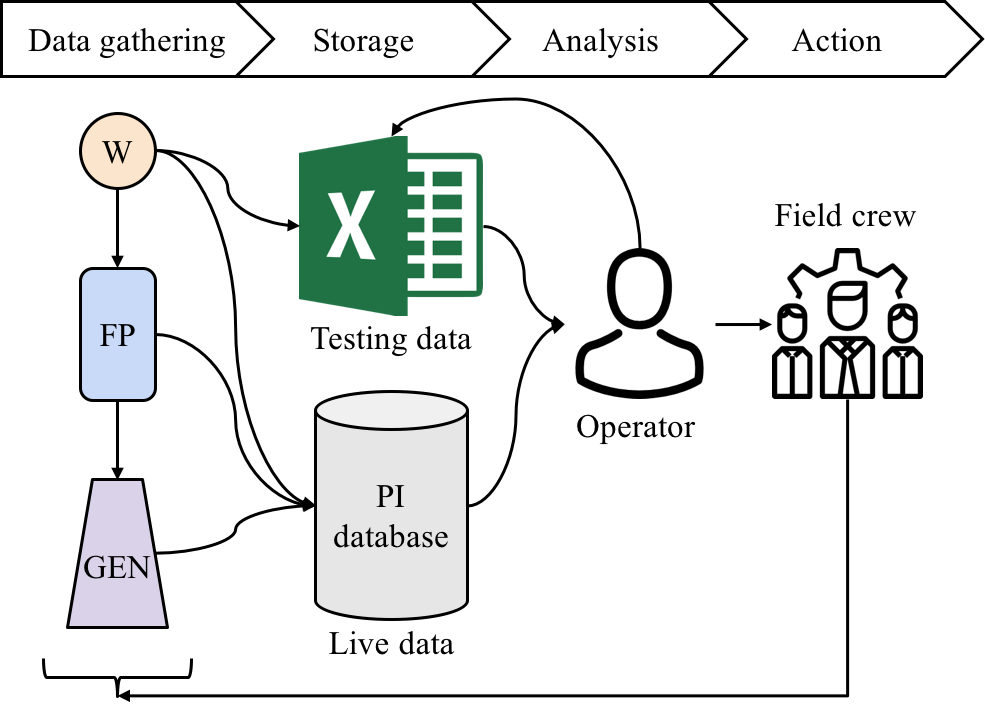
\includegraphics[width=\linewidth]{media/current_system}
  \captionof{figure}{Current system diagram. Data on the surface network components (wells, flash plants and generators) is stored in two systems, which an operator reconciles to build a model.}
  \label{fig:current_system}
\end{minipage}\hfill
\begin{minipage}[t]{.48\textwidth}
  \centering
  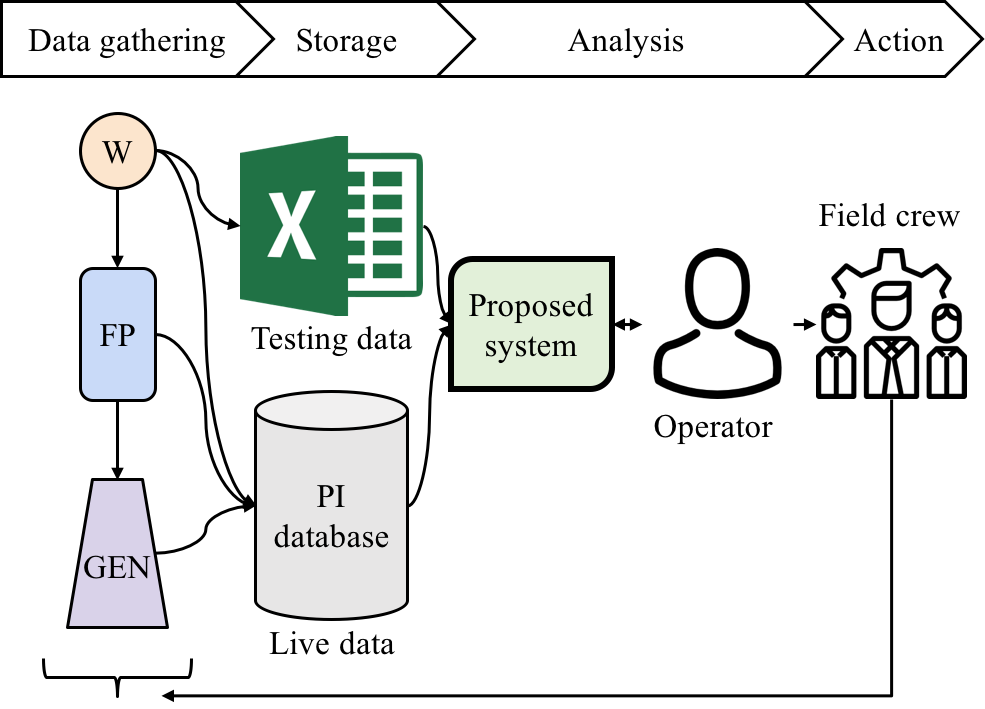
\includegraphics[width=\linewidth]{media/proposed_system}
  \captionof{figure}{Proposed system, which ingests data from both sources, incorporates it into a model and interacts with the operator to test scenarios and make predictions.}
  \label{fig:proposed_system}
\end{minipage}
\end{figure}

Contact Energy Ltd. (CEL), the operator of the Wairakei geothermal field, records a combination of field tests and live data to monitor the state of the geothermal surface network. Staff use the data to make operational decisions about well maintenance, valve positions and long-term sustainability. Currently, the flow of information in this system looks like Figure \ref{fig:current_system}. Data from flow meters and well tests is stored for analysis by an operator, who manages the maintenance and operation of the field. 

One of the major pain points is between the storage and analysis stages. To access the PI database, the operator exports data into an Excel spreadsheet. They then compare it with the well test data stored in another spreadsheet.

After calibrating the test data, running regressions and making forecasts, they obtain metrics about each well's condition and make recommendations such as whether to perform a work-over to remove deposits inside the well bore. Accessing and processing the data is a highly manual task, and the sheets have become cumbersome and slow to open. Calibration requires experience to know what the values should look like, adding dependence on a single operator.

In this paper, we develop the intermediate system shown in Figure \ref{fig:proposed_system} between the data storage and operator, that integrates the two datasets and assists in the operator's tasks by automating the statistical analysis.

There are two advantages to our proposed system:
\begin{enumerate}
\item Data from multiple sources are processed into a statistical model that includes uncertainty using Bayesian statistics.
\item The operator can interact with the internal model through Excel to conduct scenario analysis and automatically visualise the results.
\end{enumerate}

%%%%%%%%%%%%%%%%%%%%%%%%%%%%%%%%%
\section{Advantage of Bayesian Estimation}
Estimation of uncertainty is an essential part of making informative, yet realistic models. The current geothermal model used by engineers at CEL in Wairakei, north of Taupo, is deterministic. It does not take into account factors such as measurement uncertainty and parameter uncertainty when modelling the surface network of wells, pipes, flash plants and power plants. Therefore, there is a lack of understanding around how reliable the forecasts generated by the model are, and how this reliability might change in different parts of the surface network.
A new model that takes into account different sources of uncertainty, from errors in model parameters to errors in measurements, lends itself to Bayesian techniques. 

Historically, the main barrier to Bayesian statistics was the computational cost of calculating posterior distributions. In frequentist statistics, the use of approximations allows standard distributions (e.g. the exponential family, notably the Normal distribution) to be used. Many problems with Normal distributions have analytic solutions and are therefore cheap. An example is the Central Limit Theorem for large data sets, where the average of n independent samples converges to a Normal distribution.

With Bayesian statistics, no such assumptions are made. The key components of Bayesian statistics are three functions: a prior distribution, a likelihood function and a posterior distribution. The prior is an expert/modeller's initial belief of what the model parameters could be, before seeing any data. The likelihood function is the statistical likelihood of observing the data given any parameter value drawn from the prior, and this is used to update the prior to create the posterior, the probability of the parameter values given both the expert knowledge and the observed data. Computing the posterior is the goal, and it can either be done analytically or through simulation.

In our network model, deterministic and/or stochastic operations occur at nodal facilities such as wells, flash plants and generators.

The proportional Bayes formula is:
\begin{equation}
f(\theta|x) \propto f(x|\theta)f(\theta)
\end{equation}
where $f(\theta|x)$ is the posterior distribution of the parameters $\theta$ given the data $x$, $f(x|\theta)$ is the likelihood function of the observed data $x$ given $\theta$, and $f(\theta)$ is the prior distribution of $\theta$. The modeller selects a prior distribution based on their prior beliefs about the parameters. For example:

\begin{enumerate}
\item If it is known that $\theta_i \in [0,1]$, a Beta prior would be appropriate as it is non-zero on the interval $[0, 1]$. 
\item If a parameter resides in some ballpark due to expert knowledge, a Normal distribution may be chosen, with a variance determined by the expert's knowledge.
\item Or, if there is no prior knowledge, this is often represented by a uniform prior $f(\theta)\propto 1$, where any real value is equally likely.
\end{enumerate}

In some cases, these distributions can be chosen using true prior knowledge. Measurement uncertainty is often known to some degree, with some meters rated as having a standard error, $\sigma$, of 5 units [REF]. Therefore, we set $f(\sigma^2)$ as an Inverse-Gamma prior on measurement error with a mode of $5^2$. This is the preferred method because it satisfies the Bayes formula, where the prior is selected before observing the data.

The advantage of Bayesian statistics is that the posterior distribution represents the belief of the true network parameters after specifying both expert information and observing the data. Bayesian credible intervals also have an intuitive interpretation, compared to the Frequentist confidence interval. We use the term `credible interval' whenever the Bayesian interpretation is used (e.g. parameter estimates), and `confidence interval' for Frequentist interpretations (e.g. the T-test).

\begin{table}[ht]
\centering
\begin{tabularx}{\linewidth}{rXX}
\hline
 & Frequentist & Bayesian \\ 
  \hline
Parameter $\theta$ & Fixed by a null hypothesis $h_0$ & Random and unknown \\\hline
Data $\vec{x}$ & Random; we observe a sample & Fixed; from an unknown distribution \\\hline
95\% CI & Under repeated sampling, 95\% of CIs will contain the true $\theta$ & $\theta$ has a 95\% chance of lying within the CI  \\
   \hline
\end{tabularx}
\caption{Interpretation of confidence and credible intervals.} 
\label{tab:ci}
\end{table}

By applying computational Bayesian techniques to the Wairakei geothermal surface network, we will create an algorithmic method to calibrate our model using recorded data, simulate probabilistic flows in the network and incorporate uncertainty in our predictions.

%%%%%%%%%%%%%%%%%%%%%%%%%%%%%%%%%
\section{Wairakei Network Structure}

\begin{figure}
  \centering
  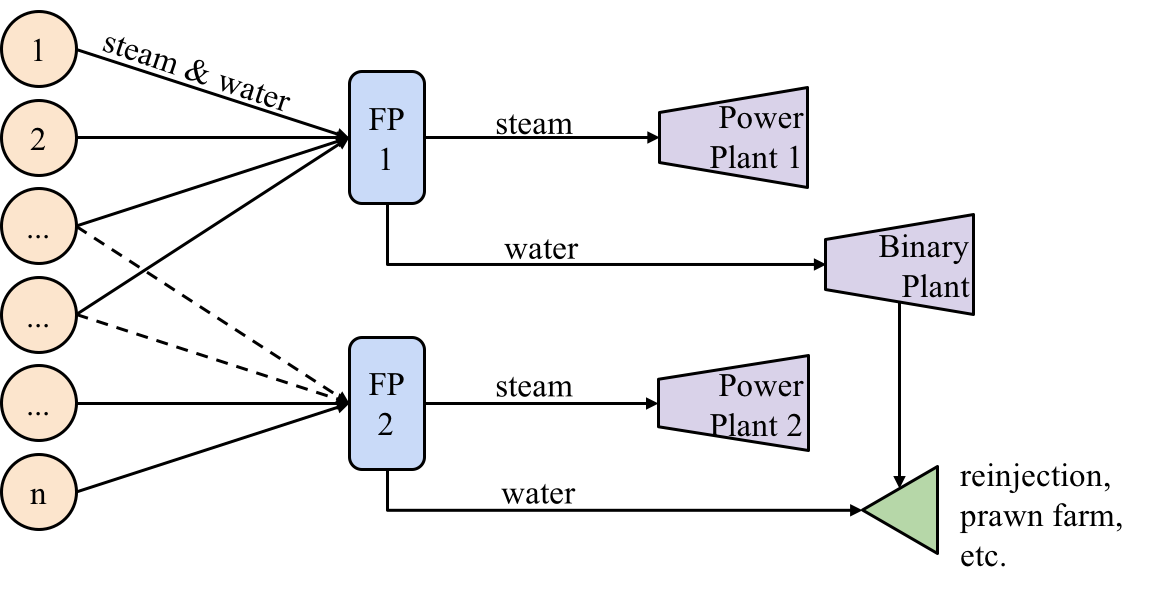
\includegraphics[width=0.5\linewidth]{media/network_diagram}
  \captionof{figure}{Simplified structure of the Wairakei geothermal surface network. Some wells can send steam to a selection of flash plants, but only one at a time (indicated by the solid/dashed lines).}
  \label{fig:network_diagram}
\end{figure}

At a single point in time, the Wairakei surface network can be represented as a directed, acyclic graph shown in Figure \ref{fig:network_diagram}. As some wells have multiple flash plants they can be routed to, the active arcs are pre-determined according to the configuration we wish to simulate.

There are three types of nodes: wells, flash plants and generators. Each node has inputs, transformations and outputs, and associated parameters.

\subsection{Well Nodes}
In the model, each well begins with an operating well-head pressure. All active wells generate mixed-phase fluid with the intensive properties of enthalpy $h_i$ and extensive properties of mass flow rate $\dot{m}_i$. Their well-head pressure is set by the operator -- note that well-head pressure is not the pressure differential between the wellbore and atmospheric. It is the pressure measured at the gauge, so zero indicates the well is at maximum flow venting into the atmosphere.

The mass flow can be predicted using wellbore simulators such as TOUGH2, but these take a long time to run and it is easier for CEL to evaluate an statistical approximation as $\dot{m} = f(\vec{x})$. CEL approximates $f$ using well test data, using three data points from a given day to fit two degrees of freedom. Often the full data set includes many sets of tests over several years.

We use their data set to calibrate a regression model with better estimations of mass flow variance by using all the data, whereas CEL fits multiple models using a small subset of the data for each. By incorporating more data, our regression model can also estimate uncertainty in its parameters.
\todo{Introduce equations}

\subsection{Flash Plant Nodes}
Flash plants take flow inputs from a partition of the set of wells, such that every (active) well maps to one flash plant in a many-to-one relationship. Configurations can come from historical records, external optimisation routines or any hypothetical setup we wish to test.

At a flash plant $j$, the extensive (mass-flow dependent) properties are summed over its subset of wells $I(j)$ and intensive (per unit mass-flow) properties are mass flow-weighted averages.
\begin{align} \
\dot{m}_j &= \sum_{i\in I(j)} \dot{m}_i\quad \forall j \label{eq:fp_mf} \\
h_j &= \frac{\sum_{i\in I(j)} \dot{m}_i h_i}{\sum_{i\in I(j)} \dot{m}_i} \label{eq:fp_h}
\end{align}
These formulae assume conservation of mass and enthalpy, which holds if network components are sufficiently sealed and insulated. Enthalpy loss in the Wairakei pipes is estimated at 0.6\% in the pipes by [REF], who concludes that it is negligible.

Impure steam from the wells causes pitting and corrosion in the generator turbines. Flash plants convert the fluid into steam with one or two pressure drops to boil the liquid component of the fluid [REF]. The resulting steam mass flow from a drop to pressure $P$ can be calculated by:
\begin{equation}
\dot{m}_{\text{steam},j} = \chi\dot{m}_j,\quad \chi= \min{\left\{\max{\left\{\frac{h_j - h_{f@P}}{h_{fg@P}}, 0\right\}}, 1\right\}}
\end{equation}
where $h_{f@P}$ is the specific enthalpy of saturated water at pressure $P$ and $h_{fg@P}$ is the latent heat of evaporation. Vapour quality $\chi$ is bounded between zero and one, and the remaining mass flow is the liquid fraction. Contact Energy has specified flow limits for different fluid outputs for each flash plant that it must stay below.

The outflowing steam and water are not constrained to go to the same generator, and several flash plants send steam to Poihipi and water to the binary plant.

\subsection{Generator Nodes}
Generators accept intermediate and low pressure steam or water from flash plants, where the subset of flash plants supplying steam to generator $k$ is $I_{\text{steam}}(k)$ and the subset of flash plants supplying water is $I_{\text{water}}(k)$. Currently, the power output $\dot{W}_k$ from a generator $k$ with efficiency $\eta_k$ is proportional to the mass flow of steam feeding it:
\begin{equation}
\dot{W}_k = \eta_k \sum_{i\in I_{\text{steam}}(k)} \dot{m}_{\text{steam},i}
\end{equation}
or
\begin{equation}
\dot{W}_k = \eta_k \sum_{i\in I_{\text{water}}(k)} \dot{m}_{\text{water},i} \label{eq:power}
\end{equation}
We are interested in the posterior distribution of total power output, $\sum_{k\in K}, \dot{W}_k$, as this is what we wish to maximise. Analysis of intermediate variables within the network gives insight into where sources of variation or uncertainty in total power output arise.

%%%%%%%%%%%%%%%%%%%%%%%%%%%%%%%%%
\section{Data Sources}
We use numerical data supplied by Contact in several forms, including network schematics, raw data and knowledge about uncertainty and limits in the field. We wish to build a production curve model and use this to make forecasts forecast, given the operating pressures for each well. A component of this project is integrating multiple data sources to predict mass flow because neither of the raw data sources covers all the wells on their own.

\subsection{Network Structure}
Contact has provided a schematic indicating the connectivity of wells, to flash plants, to generators. In some cases, wells have in-built flash plants. These are treated the same as any other flash plant, except they only have one well feeding them. When a well has the option to feed to several flash plants, the configuration is pre-determined by any operational decision.

\subsection{Well Test Data}
Well tests are recorded in an Excel spreadsheet. Wellbore tests are performed at multiple operating pressures. This allows Contact Energy to fit a production curve to the well, as discussed in the Literature Review. The spreadsheet also contains results from tracer flow tests (TFTs), which are easier and cheaper to run because the well can remain connected to the network.

Tests are only performed on the liquid wells and well-head pressure, mass flow and enthalpy are recorded manually. The liquid wells are wells with a mixed-phase fluid output, and are the main focus of this model because of their readily available data and relationship with the flash plants that separate their wet steam. \todo{Change (see David's comment)}
%What are you excluding and why? What data are missing/would be useful to collect? What are the implications of not having this data?
% (Note, these are topics that should be covered eventually, not necessarily in this section. However, as this is where you start to discuss the data, it may be a useful time to introduce the reader to data limitations?)
Missing flows from the `dry' wells (wells with integrated separators that only output steam) are covered using exported flow meter data from  CEL's automatic loggers.

\subsection{PI Flow Meters}
Real-time data is supplied using flow meters. The benefit of live data is that it is stored once a day in a PI system (treated here as a generic database) in a regular time-series containing every meter. It is therefore much more regular than the well test data. The parameters recorded include well-head pressure, separator pressure, enthalpies and mass flows for some facilities.

\todo{Better description of flow meter usage and time series}

Twenty liquid wells also have pressure gauges and flow meters logged in PI, and seventeen dry wells are not included in the liquid wells regression data. The data from the twenty wells shown in Figure \ref{fig:pi_data} is included in the production curve regression, and we include one month (thirty instances) of data to increase the weight in the regression on the most up-to-date points. We also use them to forecast the operating pressures. However, they cannot regress the production curve on their own because they tend to all be of the same well-head pressure and the regression parameter estimation would be ill-conditioned.

\begin{figure}
  \centering
  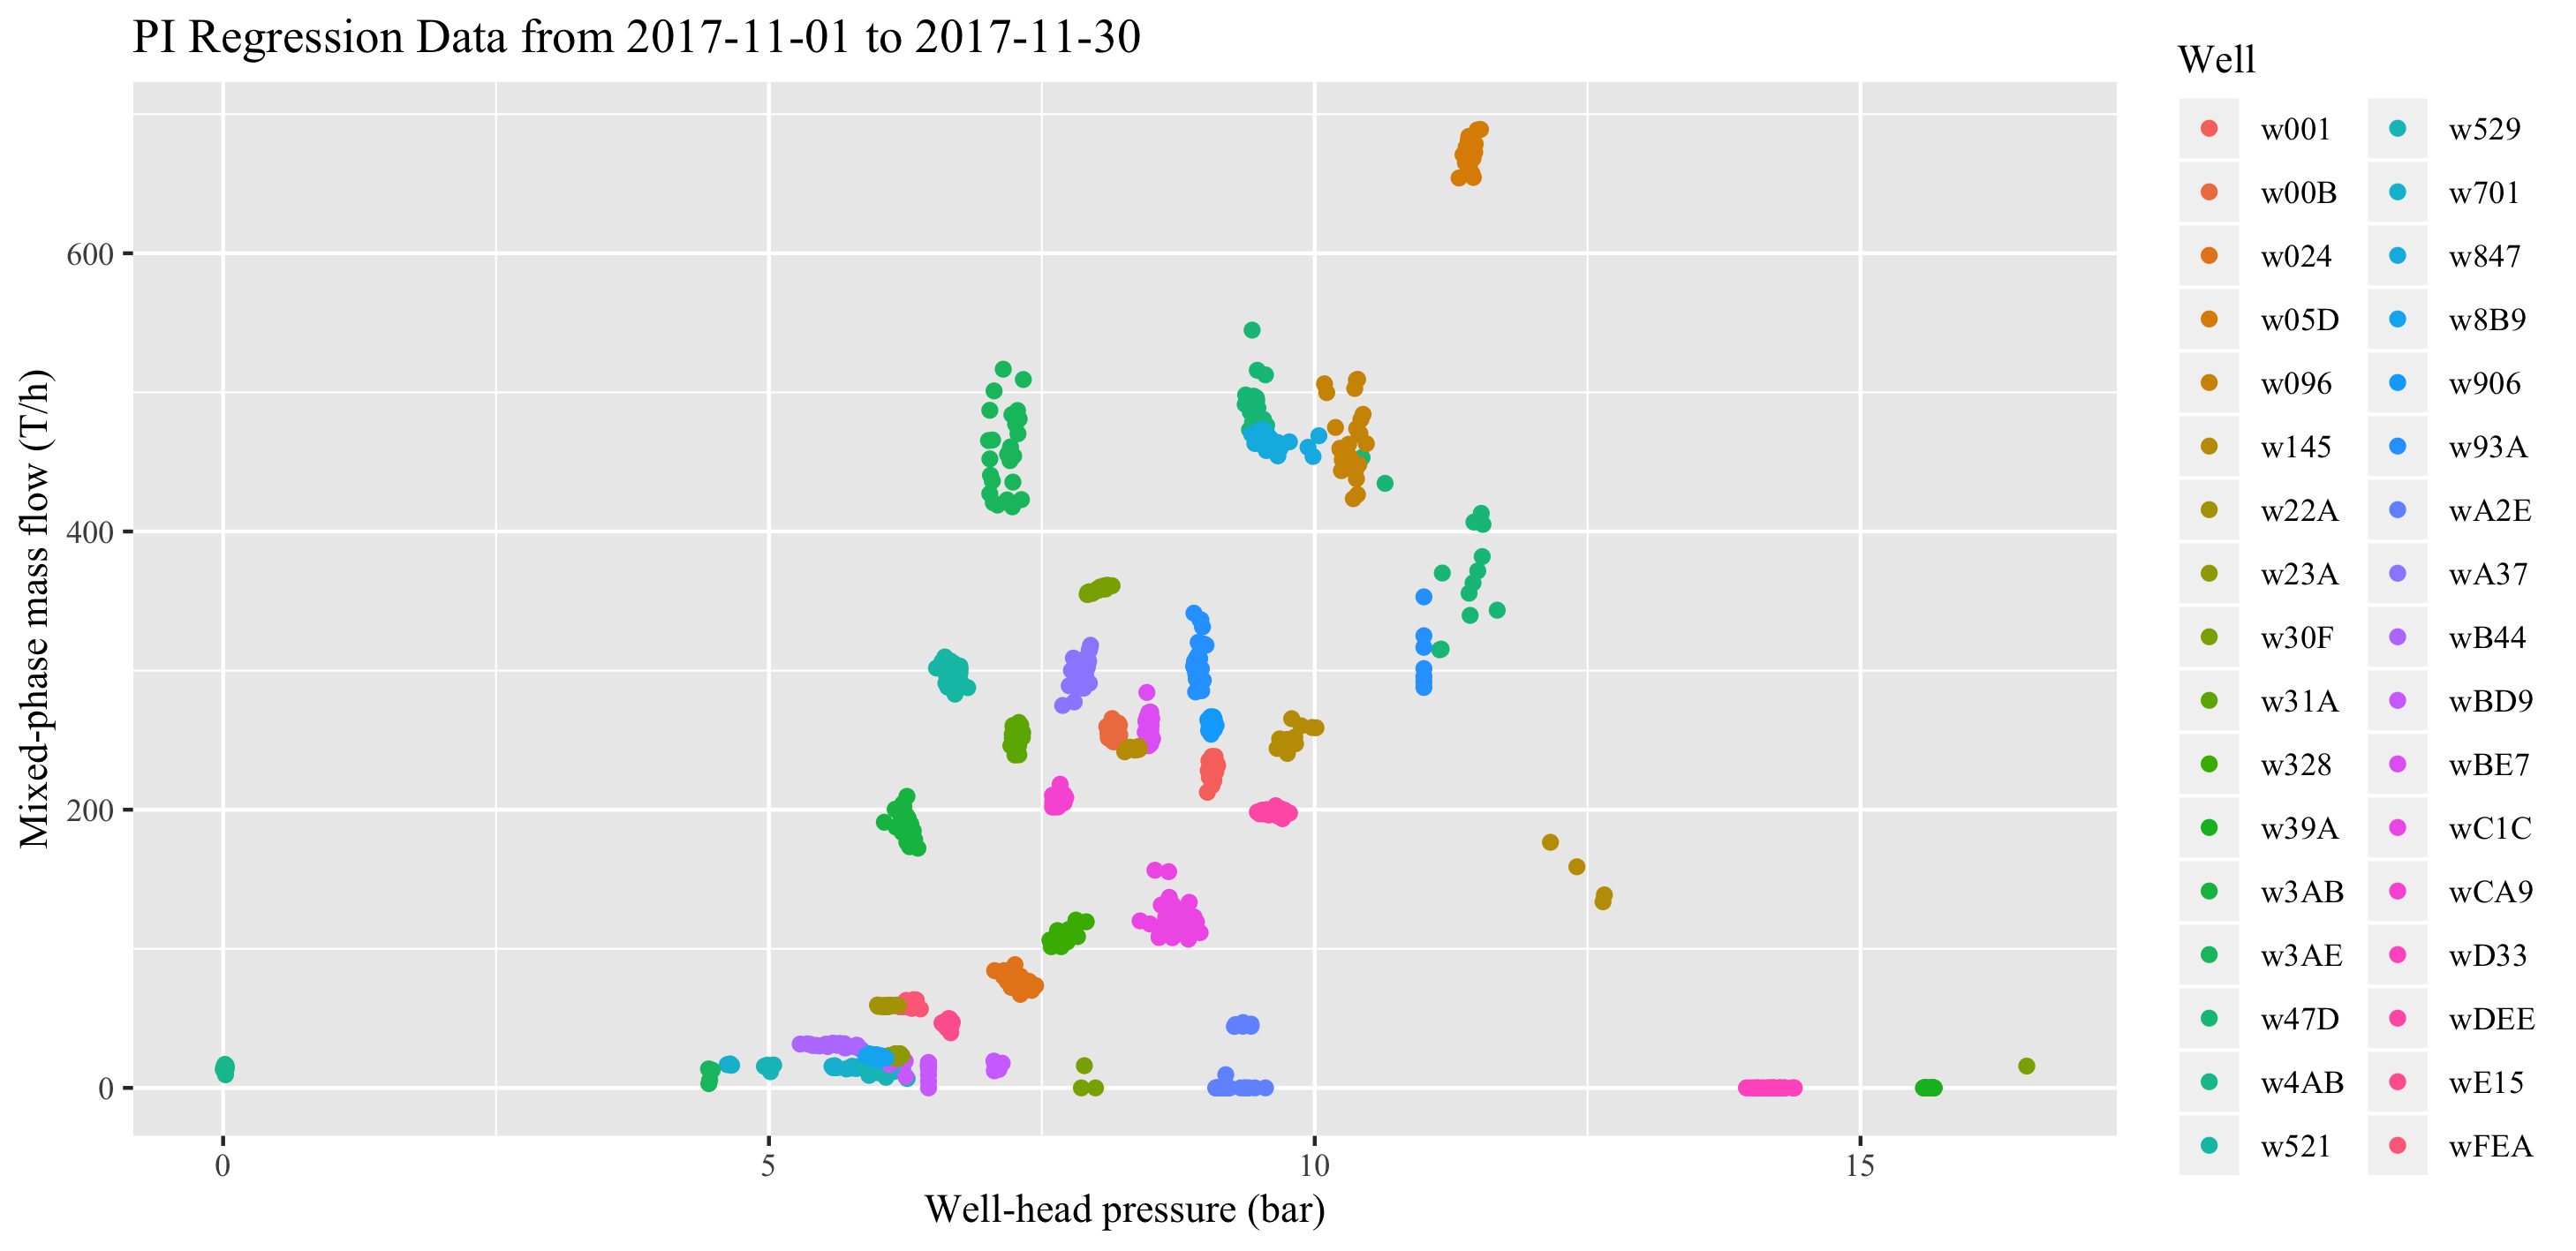
\includegraphics[width=\linewidth]{media/pi_data}
  \captionof{figure}{One month of the most recent regression data from the PI database. We use a combination of the wellbore test data (not shown) to estimate the regression parameters, and the PI data to increase the weight and precision for short-term forecasts.}
  \label{fig:pi_data}
\end{figure}

PI data is used for the ten wells without well-head pressure in a time-series analysis without a production curve. This allows us to `fill in' the gaps from the wellbore test data even though we cannot model the relationship between well-head pressure and mass flow.

\subsection{Uncertainty}
To take full advantage of the Bayesian framework, we want to specify well-informed parameters. We have obtained prior estimates for some of the measurement uncertainties by correspondence with Contact Energy:

\begin{enumerate}
\item Well test mass flow measurements are $\pm$5\%-10\%
\item Flash plant mass flow measurements are $\pm$10\%
\item Steam to power conversion factors are up to $\pm$5\%
\end{enumerate}

Turning these statements into prior specifications is to the modeller's discretion and will be discussed for the model. However, in practice most sensible priors work if there is enough data available.

\subsection{Constraint Limits}
Flash plants have a flow limit on the fluid components. This data is not a component of the Bayesian model, but can be used when analysing the outputs to check the probability of a constraint violation given a certain network configuration.
\begin{enumerate}
\item FP14 $<$ 525 T/h of IP and LP steam
\item FP15 $<$ 775 T/h
\item FP16 IP $<$ 420 T/h
\item FP16 IP+ $<$ 450 T/h
\end{enumerate}

\todo{Explain FP16 (or ignore if it isn't important}

%%%%%%%%%%%%%%%%%%%%%%%%%%%%%%%%%
\section{Data Integration}

\begin{figure}
  \centering
  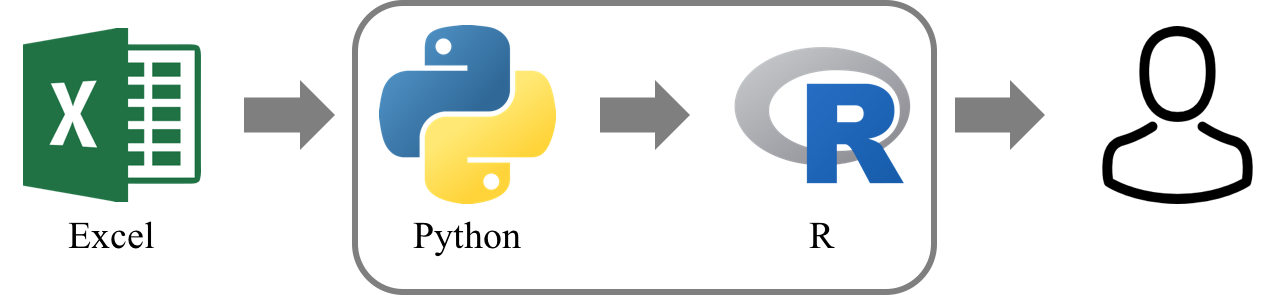
\includegraphics[width=0.5\linewidth]{media/workflow}
  \captionof{figure}{Our project includes a Python script which pre-processes the sample data files, and an R script which runs a model and processes the results.}
  \label{fig:workflow}
\end{figure}

Direct integration of our routine with Contact's PI systems was not possible for this study because of the sensitivity of live asset data. Exported Excel worksheets therefore provide the main source of data input for our implementation. This section details how we extract the raw data from provided Excel samples, how we process it and what processed data our statistical analysis requires.

\subsection{Data Extraction}
Accessing the data using the Microsoft Excel desktop application is slow, on the order of ten minutes for the sample data supplied, but much longer for the actual operational spreadsheet. Therefore, we use a Python script that accepts our unmodified data spreadsheets and immediately converts the data into efficient data frame objects. Without the overhead of Excel and the myriad of formulae within the spreadsheet, loading the data into memory from storage takes seconds.

Our Python routine implements sufficient automatic data-cleaning capabilities that fix known inconsistencies such as capital letters, reject incomplete or erroneous lines, and discriminate between data and meta-data such as comments. Data cleaning takes negligible time.

\subsection{Pre-Processing}
The original Excel spreadsheets are in human-readable formats. These include well names rather than well IDs, and lacks certain metadata such as the quantities of each facility or the mappings of wells to flash plants.

The second half of the Python script maps facility names to unique integer IDs and converts time formats into the number of days since an arbitrary baseline. These allow the data to be ingested by R. We hash all the well and flash plant names before generating outputs. Wells begin with ``W" and flash plants begin with ``FP".

We found at least one data point for 62 wells. Data was missing the following:

% latex table generated in R 3.4.2 by xtable 1.8-2 package
% Fri Sep 21 16:51:45 2018
\begin{table}[ht]
\centering
\begin{tabular}{rl}
  \hline
 & Wells \\ 
  \hline
Data available but no FP & w39A, wE1B, wCA0, w416, wD33, w675, wB31, w204, wC1A, w5F8, wA09 \\ 
   \hline
\end{tabular}
\caption{Potential data quality issues. w8F4 is known to be not connected, and wE1B has an A/B pairing with wB84.} 
\label{tab:quality}
\end{table}
\todo{What is the relationship between 26a and 26b?}

The impact of missing well data includes under-estimation of flows feeding flash plants and generators. Mass proportions at the separators may also be affected if the missing wells have extremely high or extremely low enthalpies.

\subsection{Automatic and Manual Configuration}
The rest of the workflow is carried out in R. To make the program usable to non-programmers, R reads in configuration options from a separate Excel spreadsheet. Here, the user configures the well mappings and the pressures at which they intend to operate the wells. The entire network structure can also be changed to test scenarios with different facilities.

An R script reads in the processed data and the configuration file. It uses these to construct instructions for our simulation, specifying the stochastic network's structure and parameters. R also acts as our simulation interface, performing post-processing and visualisation of the outputs.

%%%%%%%%%%%%%%%%%%%%%%%%%%%%%%%%%
\section{Simulation Methods}
When calculating a posterior density, often there is a tradeoff between flexibility and efficiency, with Markov Chain Monte-Carlo (MCMC) methods being the most flexible and analytic evaluation being the most efficient but sometimes impossible. We use a specific implementation of MCMC called JAGS through RJAGS, a package for the R language. This section details the components of JAGS used by our model.

\subsection{JAGS}

\begin{figure}
  \centering
  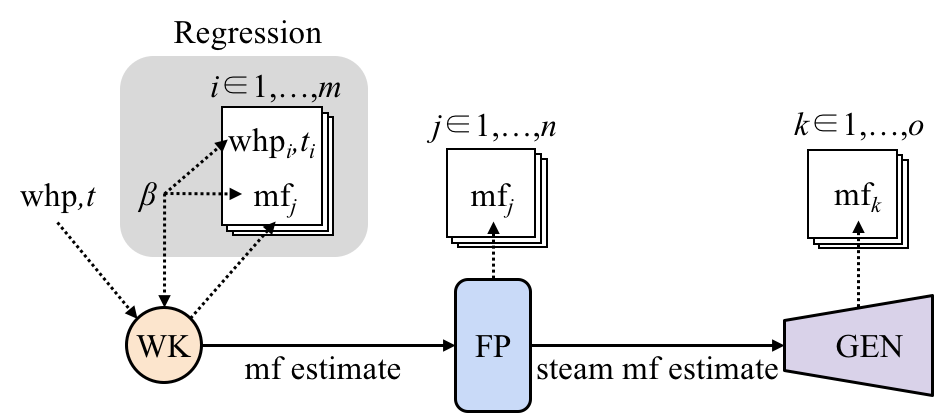
\includegraphics[width=0.5\linewidth]{media/jags_diagram}
  \captionof{figure}{One iteration of slice sampling, where a univariate density is sampled as a bivariate uniform density.}
  \label{fig:jags_diagram}
\end{figure}

JAGS (Just Another Gibbs Sampler) is a GNU-licensed program that implements a Markov Chain Monte-Carlo method called Gibbs sampling. The exact sub-components of its Gibbs routine are abstracted as a black-box to the user through an R-like syntax.

The statistical model we input into JAGS is a directed, acyclic graph. We then supply JAGS with priors for parameter nodes and data for any nodes with observations.

Figure \ref{fig:jags_diagram} shows the information flow between prior nodes, intermediate values and observed values. It is based on a graphical interface from a similar program, WinBUGS, where solid lines are deterministic relationships and dotted lines are stochastic relationships. Root nodes are prior distributions specified by the modeller, and leaf nodes are observations. 

%\todo{Check with Renate that this is correct}
To computationally compute the posterior, JAGS samples from the priors $f(\theta)$ at the root nodes (here, the well-head pressures \emph{whp} and regression parameters $\beta$) and propagates forward through the arcs. When a parameter value reaches a node we observe through measurements such as mass flow, the likelihood function $f(\vec{x}|\theta)$ is computed. The product of prior and likelihood $f(\vec{x}|\theta)f(\theta)$ becomes the posterior probability $f(\theta|\vec{x})$ for the set of parameter values $\theta$ in that iteration.

By computing the posterior distributions for all parameters, we extract the values of the regression coefficients and estimates for flows at any point in the network.

\subsection{Sampling Algorithms}
At run-time, JAGS automatically chooses the most appropriate algorithm for each node, so different nodes can use different methods. These methods come from separate modules -- \emph{base} JAGS and \emph{BUGS}.

Both of the following sampling methods are used in iterations of a Gibbs Sampler, which will be discussed afterwards.

\subsubsection{BUGS::Conjugate}
The conjugate sampler in the BUGS (Bayesian inference Using Gibbs Sampling) module is used when a parameter's posterior is a conjugate distribution to the prior. Conjugate distributions are where the posterior $f(\theta|x)$ and the prior $f(\theta)$ come from the same family of distributions. This holds when the prior is the conjugate prior to the likelihood $f(x|\theta)$.

The conjugate distributions (priors and posteriors) used in this model are the Normal and Gamma distributions, when the likelihood is a Normal distribution.

Conjugate priors and likelihoods are used wherever possible because the resulting posterior can be calculated analytically. For example, if we have the likelihood of a parameter as $f(\vec{x}|\mu,\sigma^2)\sim N(\mu,\sigma^2)$ where the conjugate prior distributions on mean and variance are $N(\mu_0,\sigma^2_0)$ and $\text{Inv-}\gamma(\alpha,\beta)$ respectively, we can calculate the analytic posterior for the individual parameter assuming the other is fixed:
\begin{align}
f(\mu|\vec{x},\sigma^2) &\sim N\left( \frac{1}{\frac{1}{\sigma^2} + \frac{n}{\sigma^2}} \left( \frac{\mu_0}{\sigma^2_0} + \frac{\sum\vec{x}}{\sigma^2} \right) , \left( \frac{1}{\sigma^2_0} + \frac{n}{\sigma^2} \right)^{-1} \right)\\
f(\sigma^2|\vec{x},\mu) &\sim \text{Inv-}\gamma \left( \alpha+\frac{n}{2} , \beta+\frac{\sum(\vec{x}-\mu)^2}{2} \right)
\end{align}
Note that in JAGS, the Normal distribution is often parameterised by precision $\tau = 1/\sigma^2$ rather than variance, leading to a Gamma conjugate prior instead of Inverse-Gamma.

Once the posterior parameters are obtained, samples are obtained by a range of methods often specific to one distribution family such as the Box-Muller method, an efficient method for transforming independent uniform (pseudo) random variates into standard Normal samples.

\subsubsection{base::Slice}
In our model, a Slice Sampler is used for all other parameters in the model that do not use conjugate distributions. The principle of slice sampling treats a univariate density as a uniform bivariate density, with one of the variates giving the same steady-state posterior as the original univariate.

\begin{figure}
  \centering
  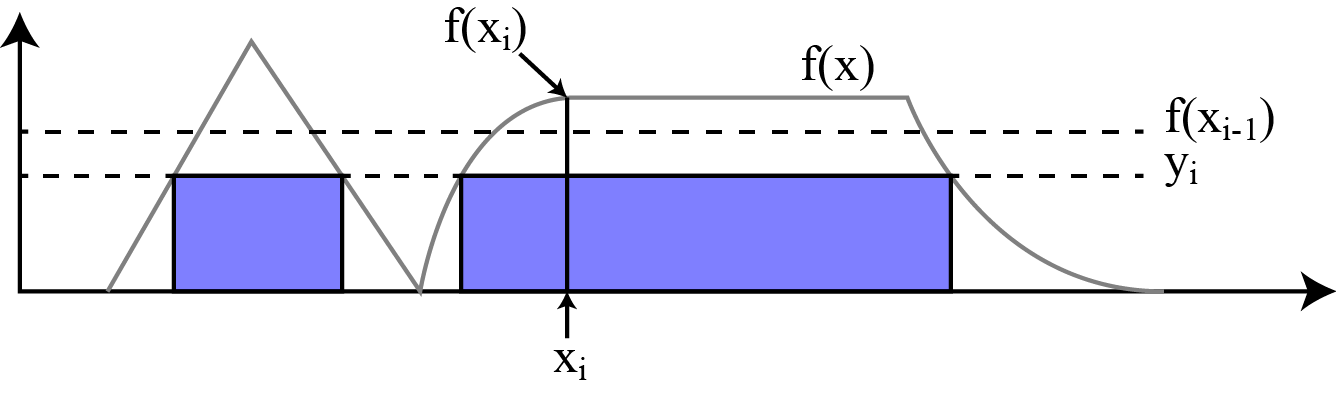
\includegraphics[width=0.5\linewidth]{media/slice_sampling}
  \captionof{figure}{A single iteration of slice sampling where a bivariate MCMC state space is constructed from a univariate density.}
  \label{fig:slice_sampling}
\end{figure}

The steps to take a slice sample are demonstrated in Figure \ref{fig:slice_sampling}: [REF]

\begin{enumerate}
\item Given $x_{i-1}$, sample $y_i$ uniformly from $[0, f(x_{i-1})]$.
\item Given $y_i$, sample $x_i$ uniformly from $\left\{ x | f(x) > y_i \right\}$.
\end{enumerate}

The long-run distribution of $x_i$ will converge on $f(x)$. Slice sampling can also be used for discrete variables, but our model only uses continuous parameters.

Slice sampling is a special form of random walker (Metropolis-Hastings) that is relatively simple to implement. By solving the inverse problem for the set $\left\{ x | f(x) > y_i \right\}$, we allow it to jump to any $x\in \left\{ x | f(x) > y_i \right\}$ and it avoids issues faced by other Metropolis algorithms where the random walker can become trapped by zero-valued regions .

\subsection{Gibbs Sampling}
The previous methods are all implementable as part of a Gibbs sampling algorithm. A Gibbs sampler is a MCMC (Markov Chain Monte-Carlo) method, where each iteration depends on the state of the chain in the previous iteration in a stochastic function determined by the individual samplers.

Our goal is to determine the full joint distribution of all the parameters in our model, which is much more difficult than univariate or bivariate distributions. MCMC allows us to construct an ergodic Markov chain whose equilibrium or stationary distribution converges on the full, multivariate joint distribution. If it is ergodic, it will satisfy two conditions:

\begin{enumerate}
\item The chain can explore all possible parameter states from any starting state.
\item When run to infinity, its expected state distribution is equal to the joint distribution.
\end{enumerate}

In the Gibbs sampler, each iteration consists of sampling one parameter (or a block of parameters when possible, e.g. multivariate Gaussian) given the most recent values of the other parameters. One iteration proceeds as follows, where $i$ is the iteration for $p$ variables:
\begin{align}
\theta_1^{(i)} &\sim f\left( \theta_k|\vec{x}, \theta_2^{(i-1)}, \theta_3^{(i-1)},\dots, \theta_p^{(i-1)} \right)\\
\theta_2^{(i)} &\sim f\left( \theta_k|\vec{x}, \theta_1^{(i)}, \theta_3^{(i-1)},\dots, \theta_p^{(i-1)} \right)\\
&\vdots\\
\theta_p^{(i)} &\sim f\left( \theta_k|\vec{x}, \theta_1^{(i)}, \theta_2^{(i)},\dots, \theta_{p-1}^{(i)} \right)
\end{align}
This specific MCMC scheme is useful because instead of sampling from a $p$-dimensional posterior, we sample from $p$ one-dimensional posteriors. Although this means each sample is not independent as would be expected from direct sampling routines, its equilibrium state still converges to the correct distribution. The time taken to reach equilibrium depends on how well the random walkers mix within their distributions, which is why conjugate and slice samplers are effective as they do not use a fixed step-size.

% The Gibbs sampler can be proven to satisfy the MCMC conditions [REF STATS 731]. JAGS uses the its constructed Markov chain with the univariate conjugate and slice sampling methods to approximate the joint posterior distribution of the geothermal surface network.

%%%%%%%%%%%%%%%%%%%%%%%%%%%%%%%%%
\section{Simulation Implementation}
JAGS code is language-agnostic and defined using a text string, Appendix [REF]. We use R instead of similar Python packages because the R interface is better supported. The RJAGS package also includes extra model and convergence diagnostics that are not available in Python, but the model declaration is still the same in any language.

There are three main steps to running a JAGS model: model specification, post-processing and model diagnostics.

\subsection{Model Specification}
JAGS code is declarative and interpreted simultaneously. However, our code can still be interpreted as a set of steps where each block leads into the next. We begin at the wells and progress through the network to the generators.

\subsubsection{Covariate Centering}
Our code contains a generalised linear model (GLM) in Equation \ref{eq:linreg} that is incompatible with JAGS' \emph{GLM} module, a specialised sampler for GLMs that is efficient when there is covariance between the parameters. Since we cannot use the module, we center the covariates. For example:
\begin{equation}
x_\text{whp} \leftarrow x_\text{whp} - \overline{x_\text{whp}}
\end{equation}
When there is high covariance, univariate samplers mix poorly because the step of one parameter is highly dependent on the value of another parameter rather than being mostly random. Centering the covariates makes the expectation of covariance zero, and we observe better mixing afterwards.

\subsubsection{Well Production Curve Regression}
One of CEL's current tasks is to fit a model to well production curves, where mass flow is a function of well-head pressure. Production curves change over time as the well and reservoir conditions change. Grant and Bixley propose a shifted elliptic form because it has interpretable real-world parameters of a maximum pressure and a maximum mass flow.
\begin{equation}
\frac{\left( \dot{m}-\beta_1 \right)^2}{\beta_2^2} + \frac{P_\text{wh}^2}{\beta_3^2} = 1
\end{equation}
Contact Energy's existing spreadsheets use a centered ellipse, which only requires two data points to fit rather than three for the extra axis shift parameter:
\begin{equation}
\frac{\dot{m}^2}{\beta_1^2} + \frac{P_\text{wh}^2}{\beta_2^2} = 1
\end{equation}
In practice, our model is not trying to estimate maximum pressures and mass flows, since these are theoretical and are not obtained in the field [REF Grant \& Bixley]. Therefore, we are not restricted to this form of equation, and we can use a linear regression, which is accurate in the vicinity of the data when the production curve can be approximated as a first-order multivariable Taylor series.

Elliptic models have convergence issues in Bayesian regression. A potential cause is the square root operation, which is undefined for negative arguments. If we want to use a linear, non-curved model, we must check whether curvature is present in the data. Since we cannot fit an elliptic model, we add a quadratic $P_\text{wh}^2$ term to the linear model and compare the deviance information criterion (DIC), a goodness of fit measure for Bayesian models. \todo{Test or state whether we are extrapolating}

\begin{table}[ht]
\centering
\begin{tabular}{lrr}
  \hline
& Quadratic & Linear \\ 
  \hline
Mean deviance & 20805 & 20883 \\
Penalty & 144.3 & 122.1 \\
Penalised deviance & 20949 & 21005\\
   \hline
\end{tabular}
\caption{DIC comparison of two GLM candidates} 
\label{tab:curvature}
\end{table}

The quadratic model has a lower mean deviance because more the extra parameter will always fit the data better. However, the penalty on the number of effective parameters is higher. The penalised deviances of both models are on the same order of magnitude, so there is not a very large difference in fitting ability. We therefore prefer the linear model for the interpretability of its parameters.

One of our extensions on the current Contact model is to incorporate time as a covariate. This allows for estimation of the production decline over time and can forecast into the future. The equation we fit is:
\begin{equation} \label{eq:linreg}
\dot{m} = \beta_1 + \beta_2P_\text{wh} + \beta_3t + \epsilon,\quad \epsilon\sim N(0, \sigma^2)
\end{equation}
and the corresponding Normal likelihood function per data point (the full likelihood is the product of its components):
\begin{equation}
L\left( \dot{m} | \vec{\beta},\sigma^2,P_\text{wh},t \right) = \frac{1}{\sqrt{2\pi\sigma^2}} e^{-\frac{-\dot{m} + \beta_1 + \beta_2P_\text{wh} + \beta_3t}{2\sigma^2}}
\end{equation}
where $\dot{m}$ is the mass flow, $P_\text{wh}$ is a specified well-head pressure, $t$ is a specified number of days after a baseline, and $\epsilon$ is a Normally distributed error of unknown variance. This form has several benefits over the other models considered:

\begin{enumerate}
\item Coefficients are interpretable as rates of change, rather than theoretical maximum limits in the elliptical model.
\item A simpler model with fewer parameters is less likely to over-fit to the data.
\item There are no root or power operations. Sampling is significantly faster (~5x).
\end{enumerate}

This model assumes the trend in the relationship is linear with time, the same assumption currently made by CEL in their spreadsheets. We also assume a stationary distribution of independent errors $\sigma^2$, which are a product of measurement errors and flow variance. We derive a prior for the measurement error from CEL, and sample from flow variance when we make predictions. In cases where $P_\text{wh}$ is unavailable, such as from the PI database, we drop the $\beta_2P_\text{wh}$ term, leading to the assumption that $P_\text{wh}$ is constant. This assumption is true as long as there is no change in back-pressure in the network from a configuration change, and the condition of the well is steady between the measurements and the time of prediction.

We monitor the traces of the regression parameters to gather statistical estimates for mass flow decline over time $\beta_3$ and flow variance.

We use a hierarchical Bayes structure to set priors on the regression coefficients $\vec{\beta},\tau=1/\sigma^2$, where $\tau$ is precision and is often used because it makes the analytic calculations simpler. Rather than making every individual parameter non-informative, we use the assumption that parameters between wells come from the same (unknown) distribution:
\begin{align}
\beta_i &\sim N\left( \mu_{\beta_i},\tau_{\beta_i} \right)\\
\tau &\sim \gamma\left(\alpha_\tau,\beta_\tau\right)
\end{align}
where the hyper-parameters have an non-informative prior, $f\left(\mu_{\beta_i},\tau_{\beta_i},\alpha_\tau,\beta_\tau\right) \propto 1$.
 
This is physically motivated because:

\begin{enumerate}
\item For $\beta_3$, pressure loss over time affects multiple wells.
\item For $\beta_1$ and $\beta_2$, wells in a field may have similar production curves.
\end{enumerate}

This is not the same as saying the parameters between the wells are identical. Instead, it fits a distribution of well production curves from which each well is observed.

The biggest benefit of this added bias is the reduction in variance for wells with insufficient or no data. We instead make an educated imputation that their production curve is similar to the wells we have data for, rather than having absolutely no imputation at all.

Our regression model is supported by the diagnostic plots of observed mass flows against fitted mass flows, and a standardised residual plot using residuals:
\begin{equation}
\epsilon_\text{std} = \frac{\hat{\dot{m}} - \dot{m}}{\text{sd}\left( \hat{\dot{m}} \right)}
\end{equation}
where $\hat{\dot{m}}$ is sampled from the Bayesian regression.

A well-fitting regression shows a linear correlation between the fitted and observed values. If we believe the residuals are Normally distributed, the standardised residual plot will have a standard Normal distribution for all the fitted values. 

\begin{figure}
\centering
  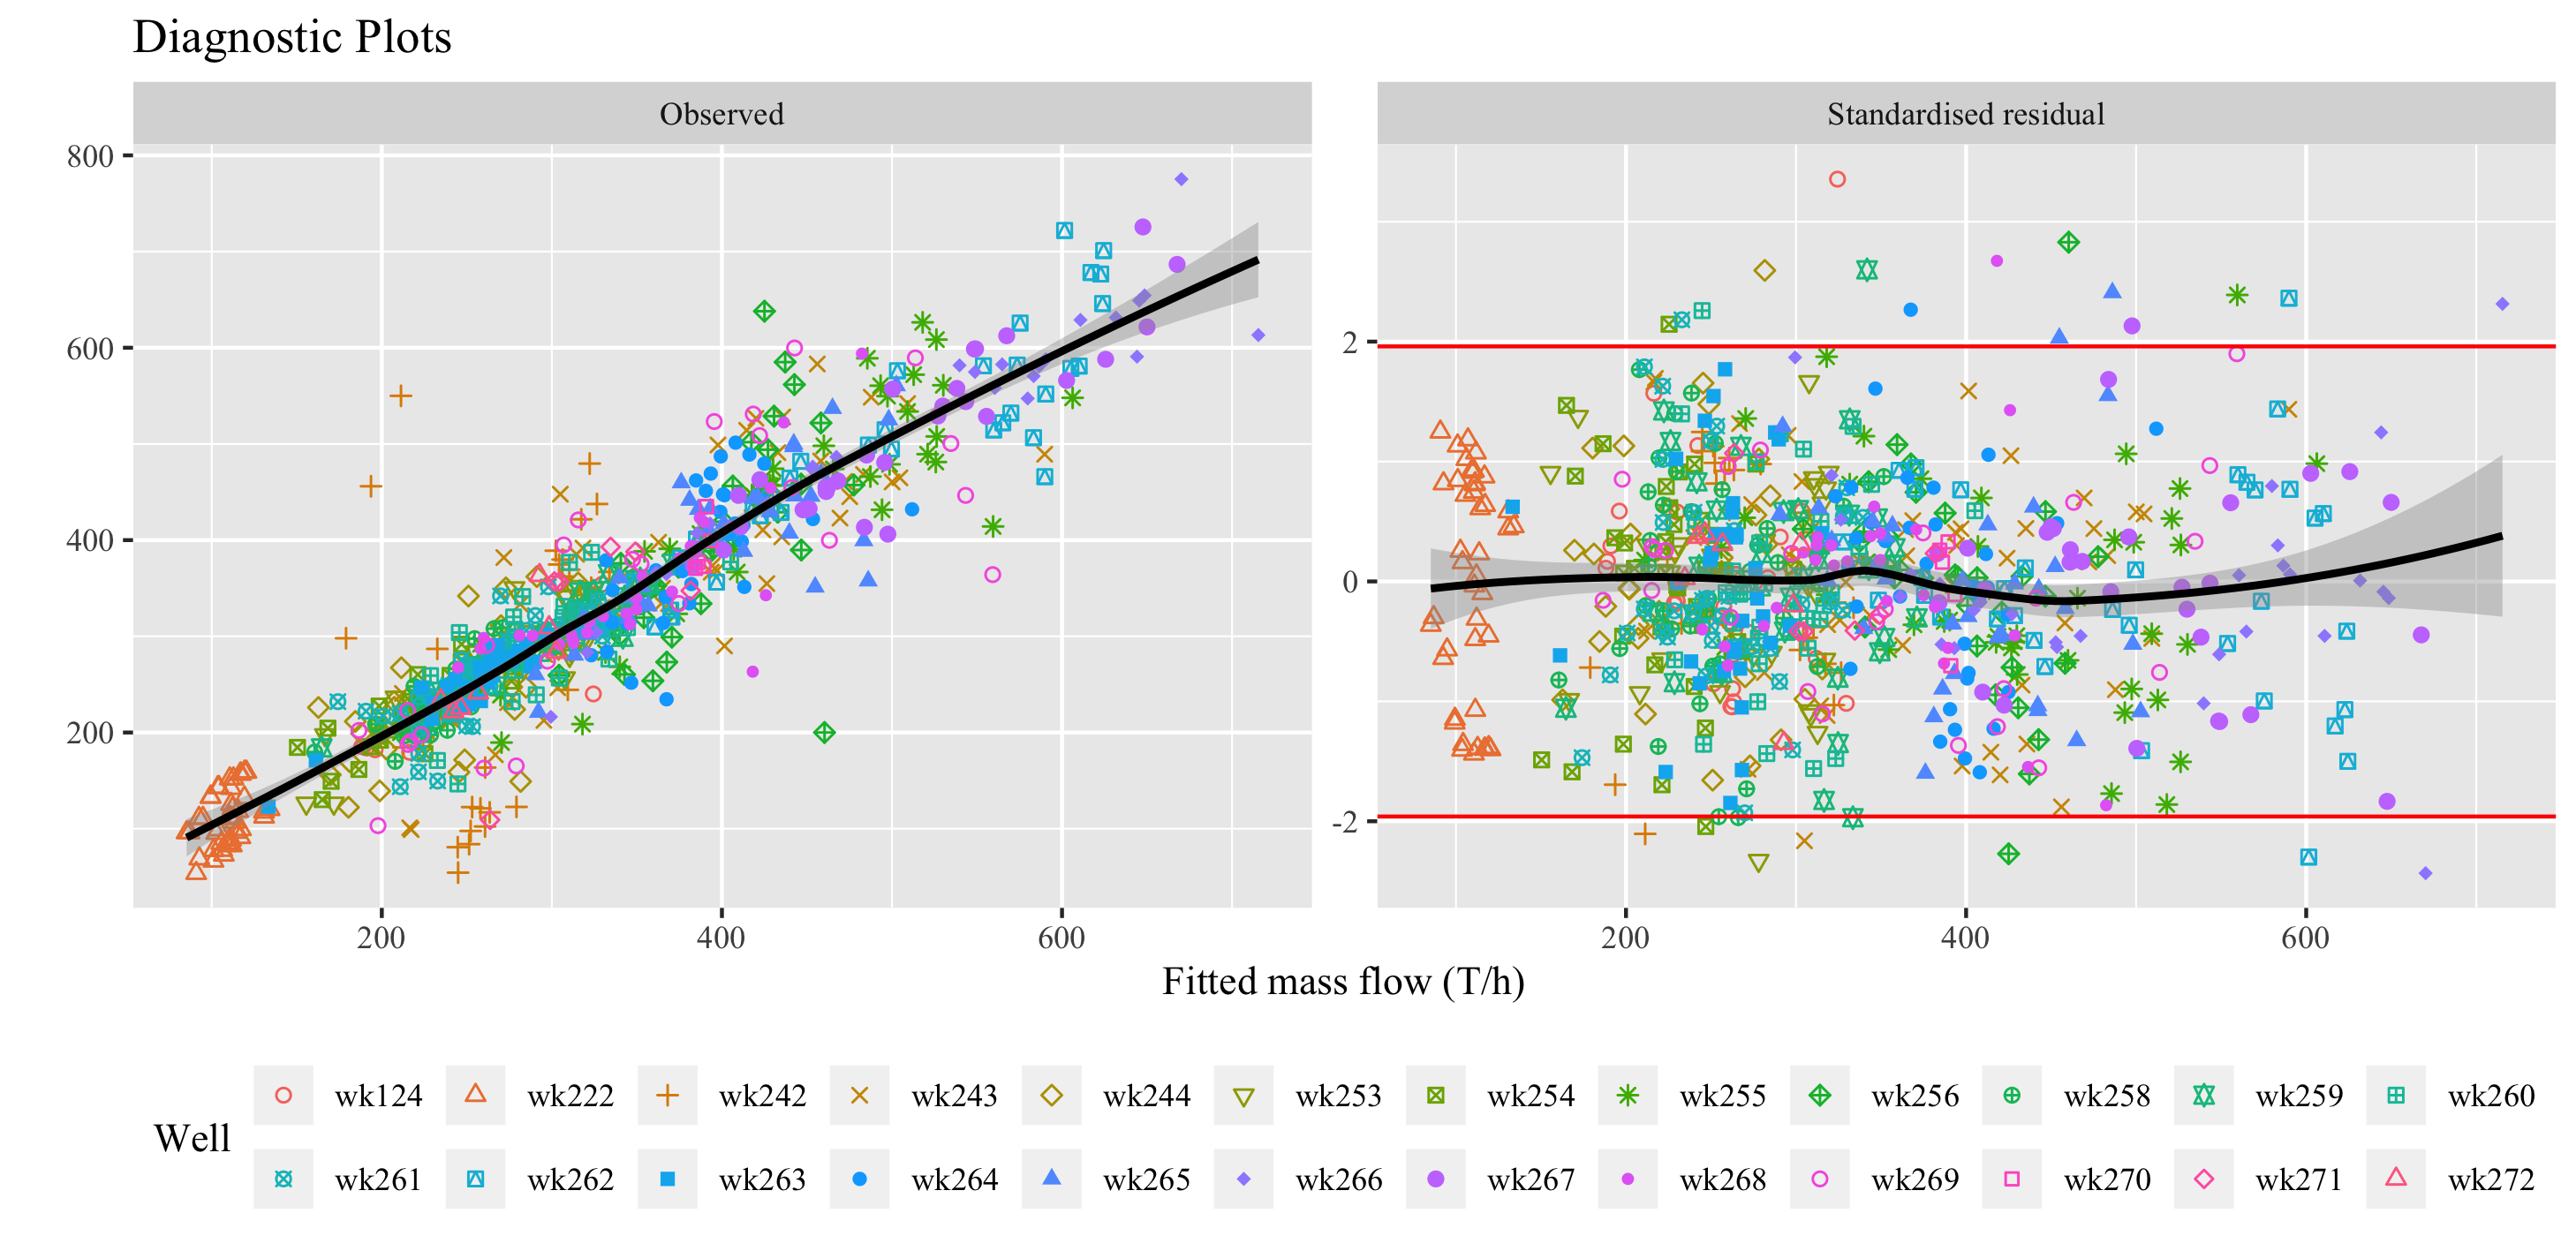
\includegraphics[width=\linewidth]{media/diagnostics}
  \captionof{figure}{Diagnostic plots with the observed response against fitted values, and residuals against fitted response. These diagnostics suggest a good fit to the data.}
  \label{fig:diagnostics}
\end{figure}

In Figure \ref{fig:diagnostics}, there is good correlation in the Observed $\sim$ Fitted plot and standardised residuals are roughly symmetrically distributed. %The residual plot also validates our implementation of errors, where the observed variance is $\sigma^2$ multiplied by a measurement error of $<$10\%. The standardised residuals become significantly inflated without this.
% CHANGE ABOVE
\todo{Comment on residual error?}

\subsubsection{Prediction}
With posterior production curves fitted for most wells, e.g. Figure \ref{fig:production_curve}, we can estimate the mass flows at a given well-head pressure and date, specified in the configuration file. We also assign a measured enthalpy to the well flows, or apply a hierarchical posterior to any missing enthalpy values. Wells without production curves are imputed using a time-series on the PI data -- see Figure \ref{fig:ts_experiment} for examples of the time series regression.

Figure \ref{fig:full_network} shows the modelled connectivity between wells, flash plants and generators. Dummy generators have been added so that a flash plants can send one type of flow (e.g. intermediate pressure steam) to one generator, and another (e.g. water) to a second generator.

\subsubsection{Flash Plant Flows}

\begin{figure}
\centering
\begin{minipage}[t]{.48\textwidth}
  \centering
  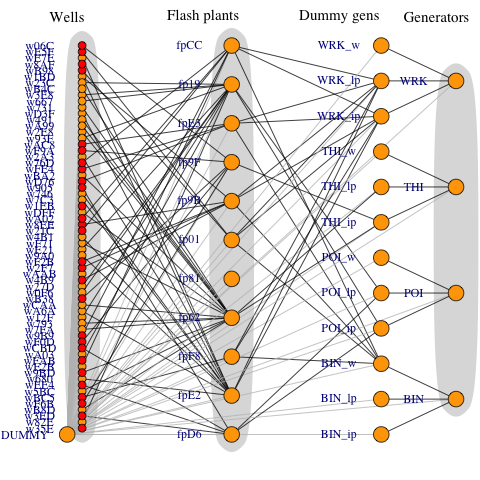
\includegraphics[width=\linewidth]{media/full_network}
  \captionof{figure}{Full network diagram, with flows from left to right. Red wells indicate forecasts have been filled in from the PI data, and dummy arcs are in grey.}
  \label{fig:full_network}
\end{minipage}\hfill
\begin{minipage}[t]{.48\textwidth}
  \centering
  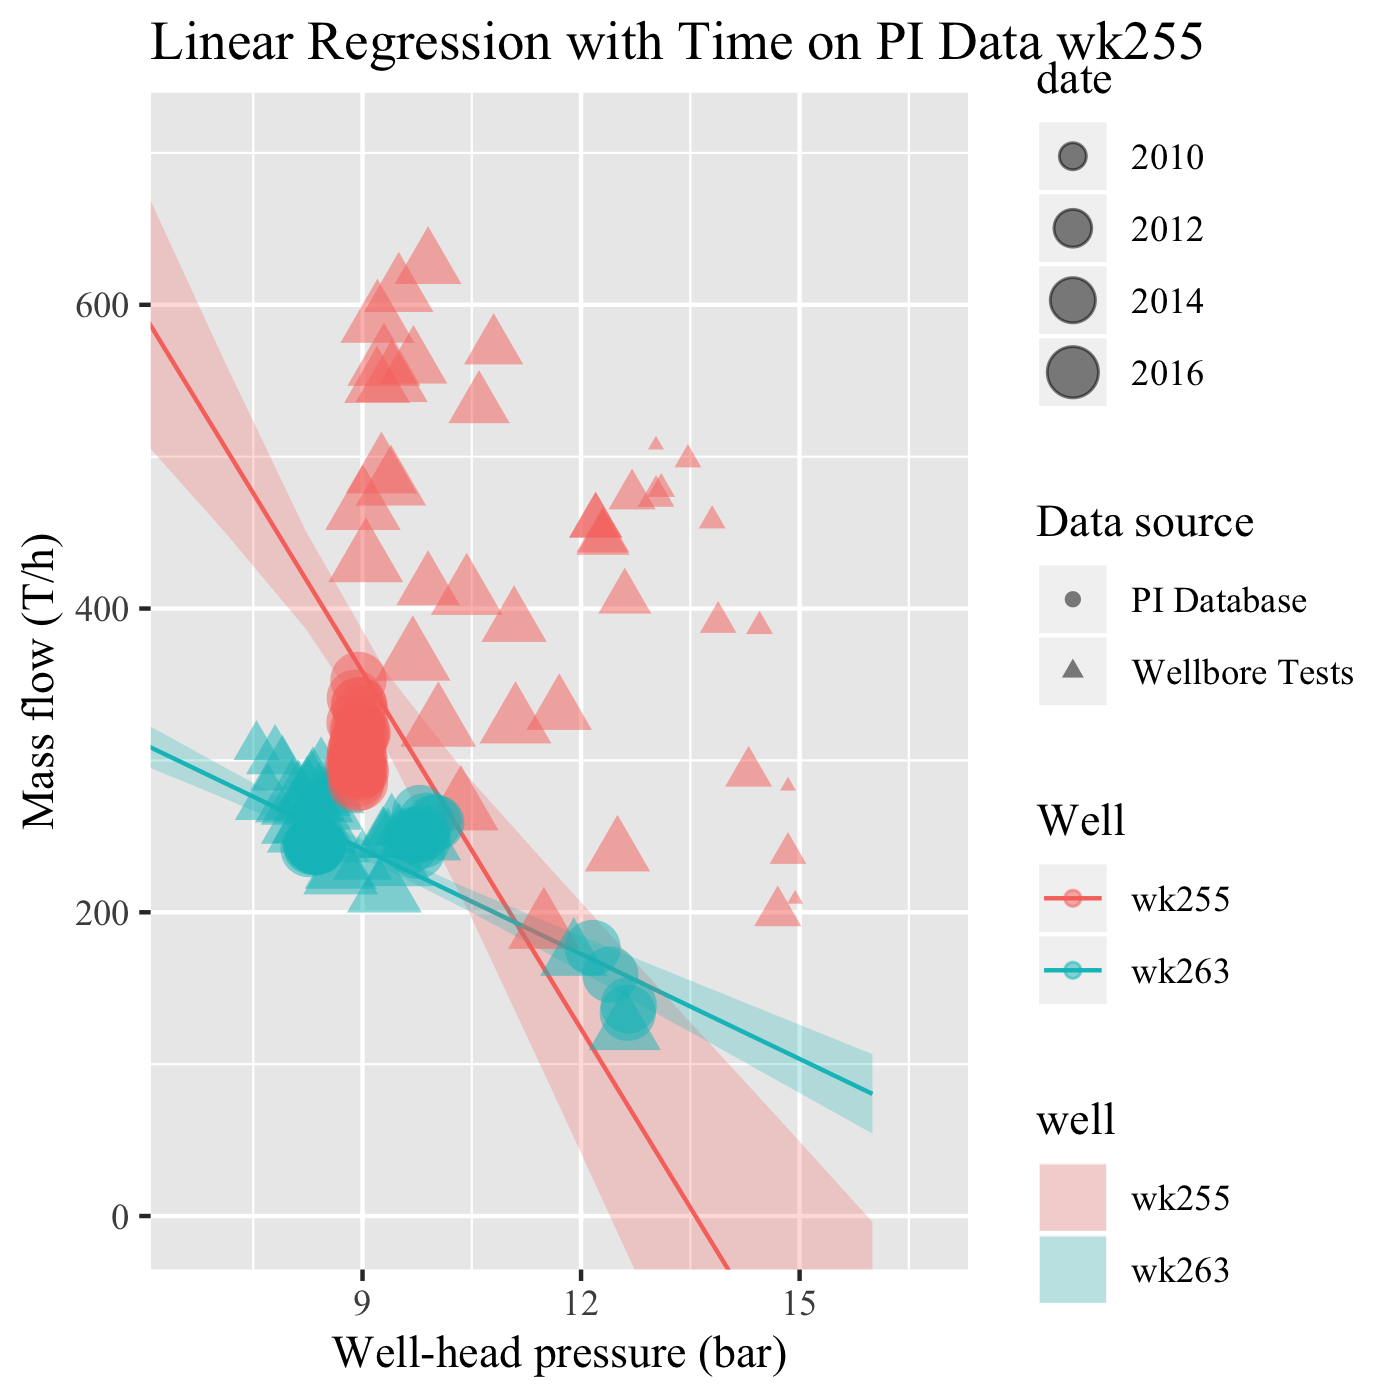
\includegraphics[width=\linewidth]{media/production_curve}
  \captionof{figure}{Two fitted production curves, forecasted one day in the future. We expect it to fit closely to the most recent data. The shaded region shows 95\% credible intervals.}
  \label{fig:production_curve}
\end{minipage}
\end{figure}

Well-to-flash-plant assignment is specified in the configuration spreadsheet. Although most well/flash-plant relationships are fixed by the physical pipes, there is a subset of wells that can swing between three flash plants, which have steam flow limits. The decisions for which wells flow to which flash plants can be optimised with a mixed-integer linear program [REF], chosen manually, or chosen by any arbitrary method.

To calculate mass flows and flow enthalpies entering a facility (both flash plants and generators), we use equations \ref{eq:fp_mf} and \ref{eq:fp_h}. During preprocessing, we add a dummy node to all $I$ to ensure that $I(j)$ is not an empty set; otherwise, JAGS throws an index error. Despite using an R-like syntax, JAGS only accepts integer indices, so generating $I(j)$ is why facilities need to be re-identified by a unique integer rather than a string. 

\subsubsection{Generator Flows and Power Conversions}
During pre-processing, three dummies per generator placed in the network before the actual aggregated power is calculated. In Figure \ref{fig:full_network}, there is a dummy for each type of fluid flow: intermediate pressure (IP), low pressure (LP), or water (W). Whether these are actually used depends on the configuration inputs. For instance, the binary \emph{BIN} plant will only ever use the \emph{BIN\_w} dummy because in reality, it is a waste to send steam to the low-efficiency binary generator.

Dummy generators flow into their respective generator. Contact Energy calculates power output as a function of the bulk mass flow by Equation \ref{eq:power}. These efficiencies are given to us in units of T/h/MW. Our uncertainty in the conversion factor is $\pm5\%$, which we interpret as $\eta \sim \text{Unif}\left( 0.95\overline\eta, 1.05\overline\eta \right)$, which holds for small ($<$10\%) percentages.

\subsection{Monitoring}

Monitors are how JAGS returns posterior samples to the user. There are three types of monitors:

\begin{enumerate}
\item Mean/variance, showing the current mean/variance of a parameter up to and including a sample. We are not interested in mean and variance because the same information can be extracted from the trace.
\item DIC (deviance information criterion), to evaluate goodness of fit of the model to the data. Although DIC can play a role in validating the model structure during development, DIC is also not a permanent part of our model once it has been validated. Also, graphical goodness-of-fit techniques are preferred because an informed user can identify specific issues such as erroneous data that would not be possible with a single value.
\item Trace, showing every sample of a parameter. We use these to sample from the stationary distribution.
\end{enumerate}

The first monitor we set is on the well regression, predicting for a range of covariates to build a picture of the production curves. Examples of these curves are shown in Figure \ref{fig:production_curve}.

Next, we monitor mass flows at each facility and their probability densities. An example of its interpretation is given in Figure \ref{fig:bayesdemo}. These estimates for uncertainty are the strength of Bayesian inference; we can sample from the posteriors at the wells and propagate our uncertainty through the network to find the uncertainties at other locations.

\begin{figure}
\centering
  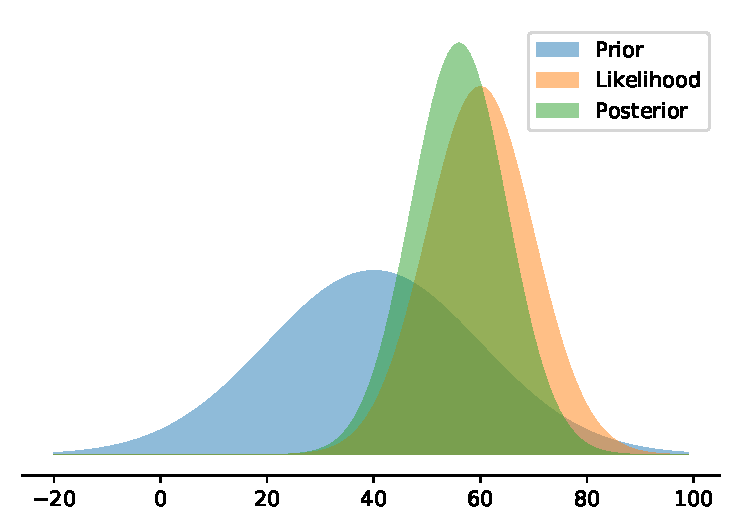
\includegraphics[width=0.5\linewidth]{media/bayesdemo}
  \captionof{figure}{The prior and likelihood functions multiply to give a posterior parameter distribution. The posterior is what we are interested in after observing the data. The uncertainty in the parameter is represented by the width of its distribution; conversely, the precision can be interpreted as the height of its peak because densities integrate to one. }
  \label{fig:bayesdemo}
\end{figure}

\subsection{Diagnostics}
One of the difficulties with MCMC approximations is they often require a burn-in (warm-up) period before settling into the stationary distribution of the Markov chain. Only the stationary distribution corresponds to the joint distribution we are interested in. In most practical uses, there is no way to predict convergence, so it must be done by monitoring the sample trace and running diagnostic tests.

\begin{figure}
\centering
  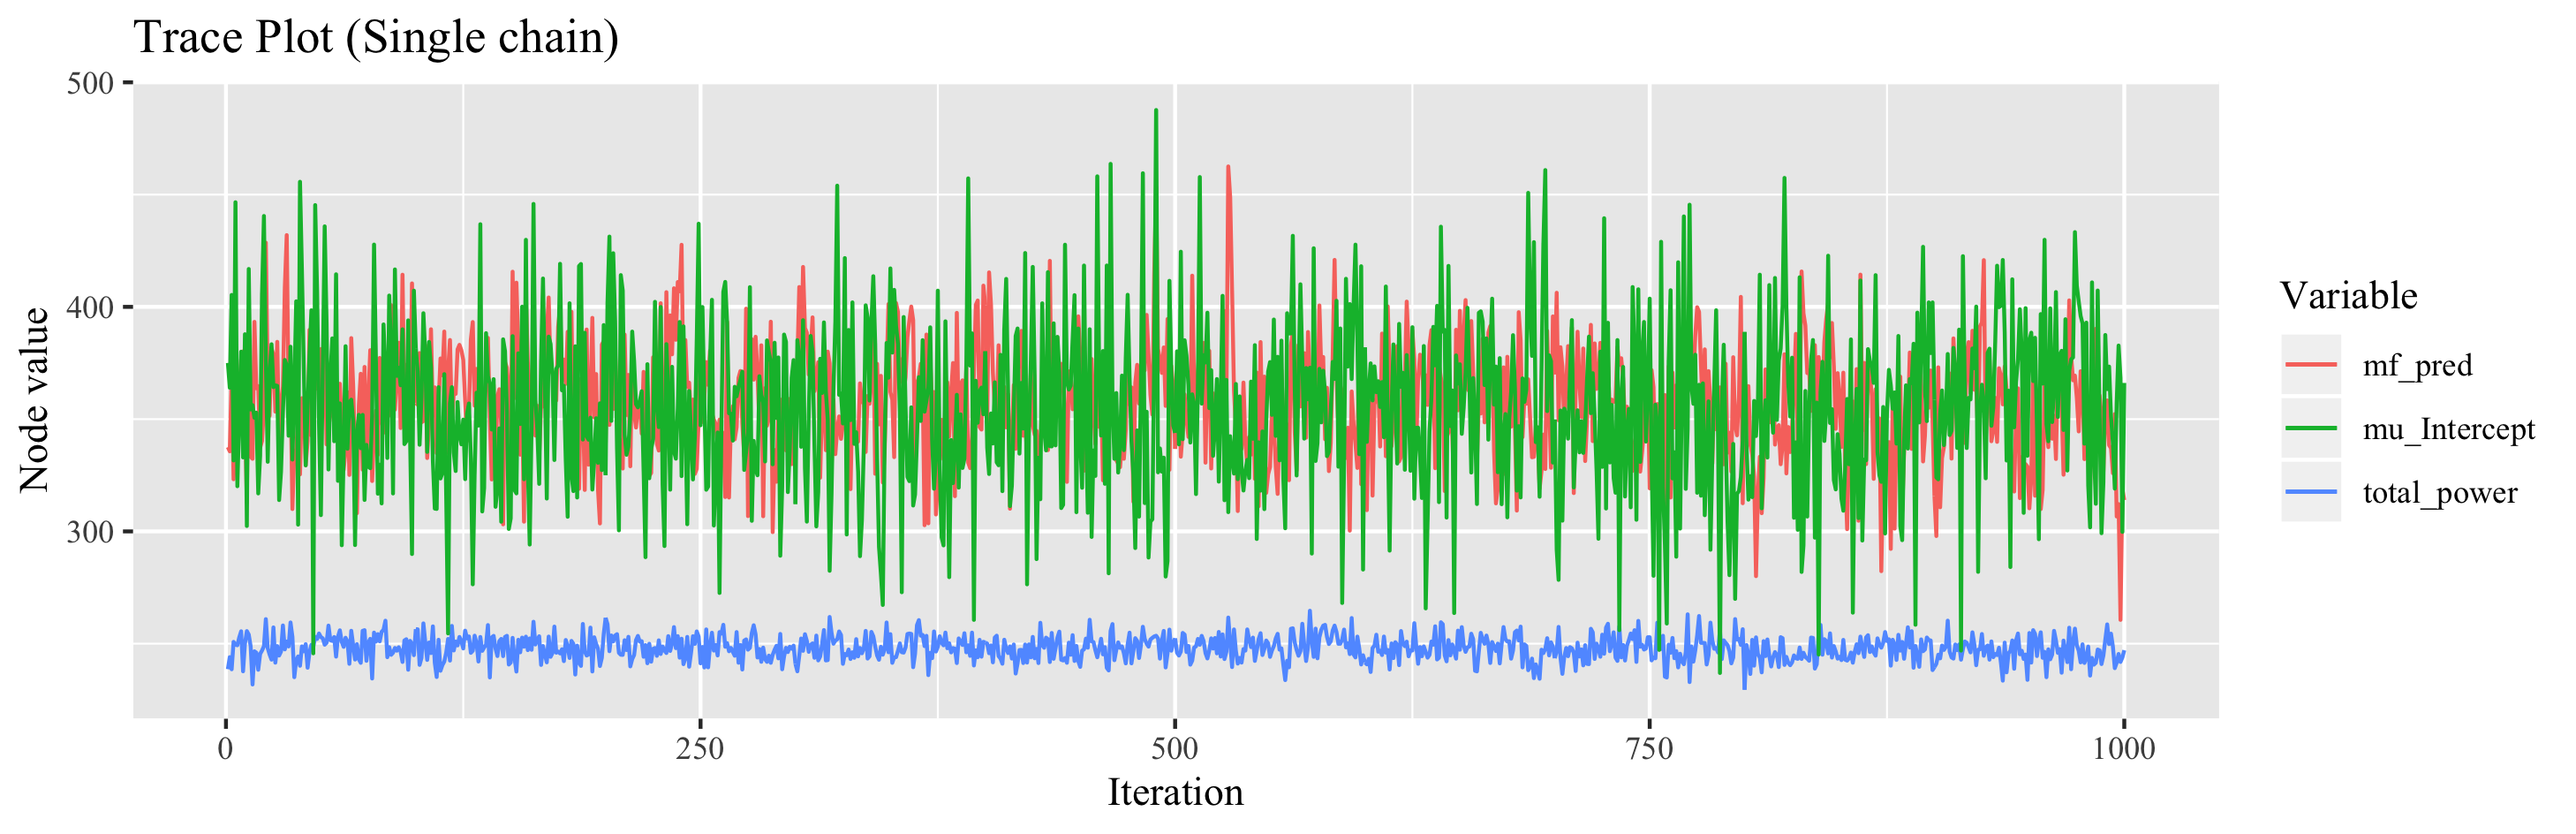
\includegraphics[width=\linewidth]{media/trace_plot}
  \captionof{figure}{Example trace plots displaying normal behaviour. The sampler appears to have reached its equilibrium distribution with no trend.}
  \label{fig:trace_plot}
\end{figure}

Poor convergence and mixing is represented by a strong trend at the beginning of the trace plot. This is not present in Figure \ref{fig:trace_plot}, but visual analysis of trace plots for every parameter.
JAGS provides other diagnostic tests in the CODA package. There are two main tests to confirm this:

\subsubsection{Geweke's Convergence}
Geweke's convergence diagnostic for MCMC samples tests for equality of the means in the first 10\% and last 50\% of the trace (the samples in iteration order). The means will be equal if the sample is drawn from a stationary distribution, indicating the burn-in period has been successfully excluded. Geweke's statistic has a T-distribution using the following T-test statistic:
\begin{equation}
T=\frac{\overline{X_1}-\overline{X_2}}{\sqrt{\frac{s_1^2}{n} + \frac{s_2^2}{m}}}
\end{equation}
where $\overline{X_1}$ and $\overline{X_2}$ are the sample means of the first 10\% and last 50\% of the samples, $s^2$ are their corresponding standard variances, and $n$ and $m$ are the number of samples in the two groups. Spectral densities are used to estimate the sample variances. [REF]. The results of Geweke's test are shown in Figure \ref{fig:geweke}.

\begin{figure}
  \centering
  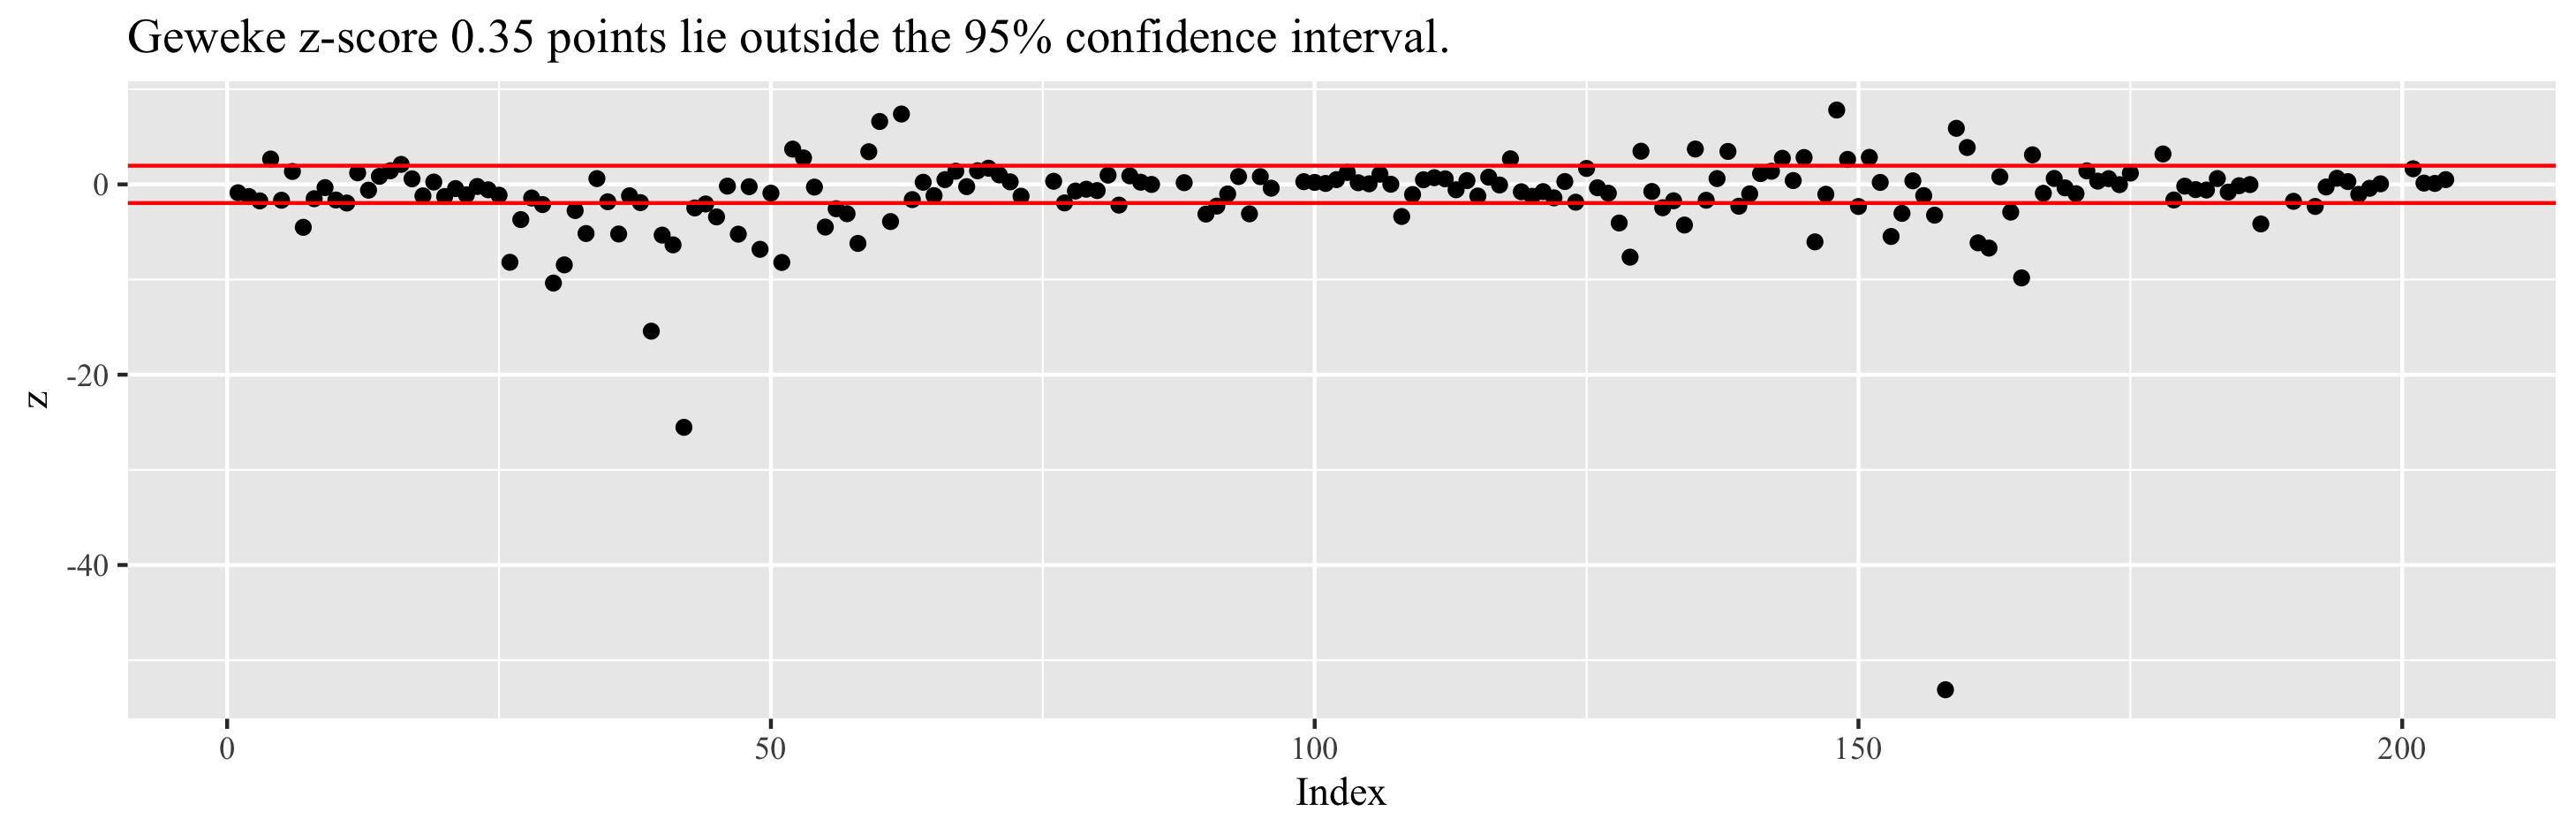
\includegraphics[width=\linewidth]{media/geweke}
  \captionof{figure}{More than 5\% of z-scores outside the confidence interval indicates the chains have not converged and are not long enough or contain burn-in.}
  \label{fig:geweke}
\end{figure}

Most of the parameters pass Geweke's test with a z-score (a Normal approximation of the T-statistic) less than 1.96 for a 95\% confidence interval. However, the changes in the power output traces were significant, so a short burn-in of 200 iterations was introduced.

\subsubsection{Gelman's Potential Scale Reduction Factor}
Gelman's test gives the potential scale reduction factor for each parameter. This requires at least two parallel chains using independent random variates (JAGS uses the Wichmann-Hill, Marsaglia-Multicarry, Super-Duper and Mersenne-Twister pseudorandom generators for the first four chains to ensure they are independent), and tests whether the chains have converged to identical distributions. If the chains have not converged, the scale reduction factors will have upper confidence limits greater than one and the samples obtained are likely to be variance-inflated and their confidence intervals may be too large. [REF]

Executing Gelman's test on all monitored parameters runs into issues with an internal Cholesky matrix factorisation of an ill-conditioned matrix. Testing a smaller selection yields Table \ref{tab:gelman}.

% latex table generated in R 3.4.2 by xtable 1.8-2 package
% Fri Sep 14 00:11:12 2018
\begin{table}[h]
\centering
\begin{tabular}{rr}
  \hline
Point est. & Upper C.I. \\ 
  \hline
1.00 & 1.00 \\ 
  1.00 & 1.01 \\ 
  1.00 & 1.01 \\ 
  1.00 & 1.03 \\ 
  1.00 & 1.02 \\ 
  1.00 & 1.00 \\ 
  1.00 & 1.02 \\ 
   \hline
\end{tabular}
\caption{Select potential scale reduction factors from Gelman's diagnostic test.} 
\label{tab:gelman}
\end{table}


Some of the upper CIs are significantly greater than one. We should be careful when interpreting any confidence intervals to do with those variables because their variance may be inflated. Running the simulation for longer will shrink the CI, but for how long is a balance between computational resources and the need for precision -- large PSRFs are acceptable if they are in components of the network that do not affect parameters of interest.

%%%%%%%%%%%%%%%%%%%%%%%%%%%%%%%%%
\section{Results}
Contact Energy has provided wellbore test data up to early 2018 and PI logs up to the end of December 31. They also supplied an example calculation for December 1st. To test the forecasting ability, we discarded all data after November 30th, 2017, and compared predicted mass flows with measured flows for December 1st. The traces were analysed in R. Because there are so many facilities and parameters to monitor, the plots in this section may only include a subset of facilities that represent the different outcomes present in the simulation.

\subsection{Mass Flows}
\begin{figure}
\centering
  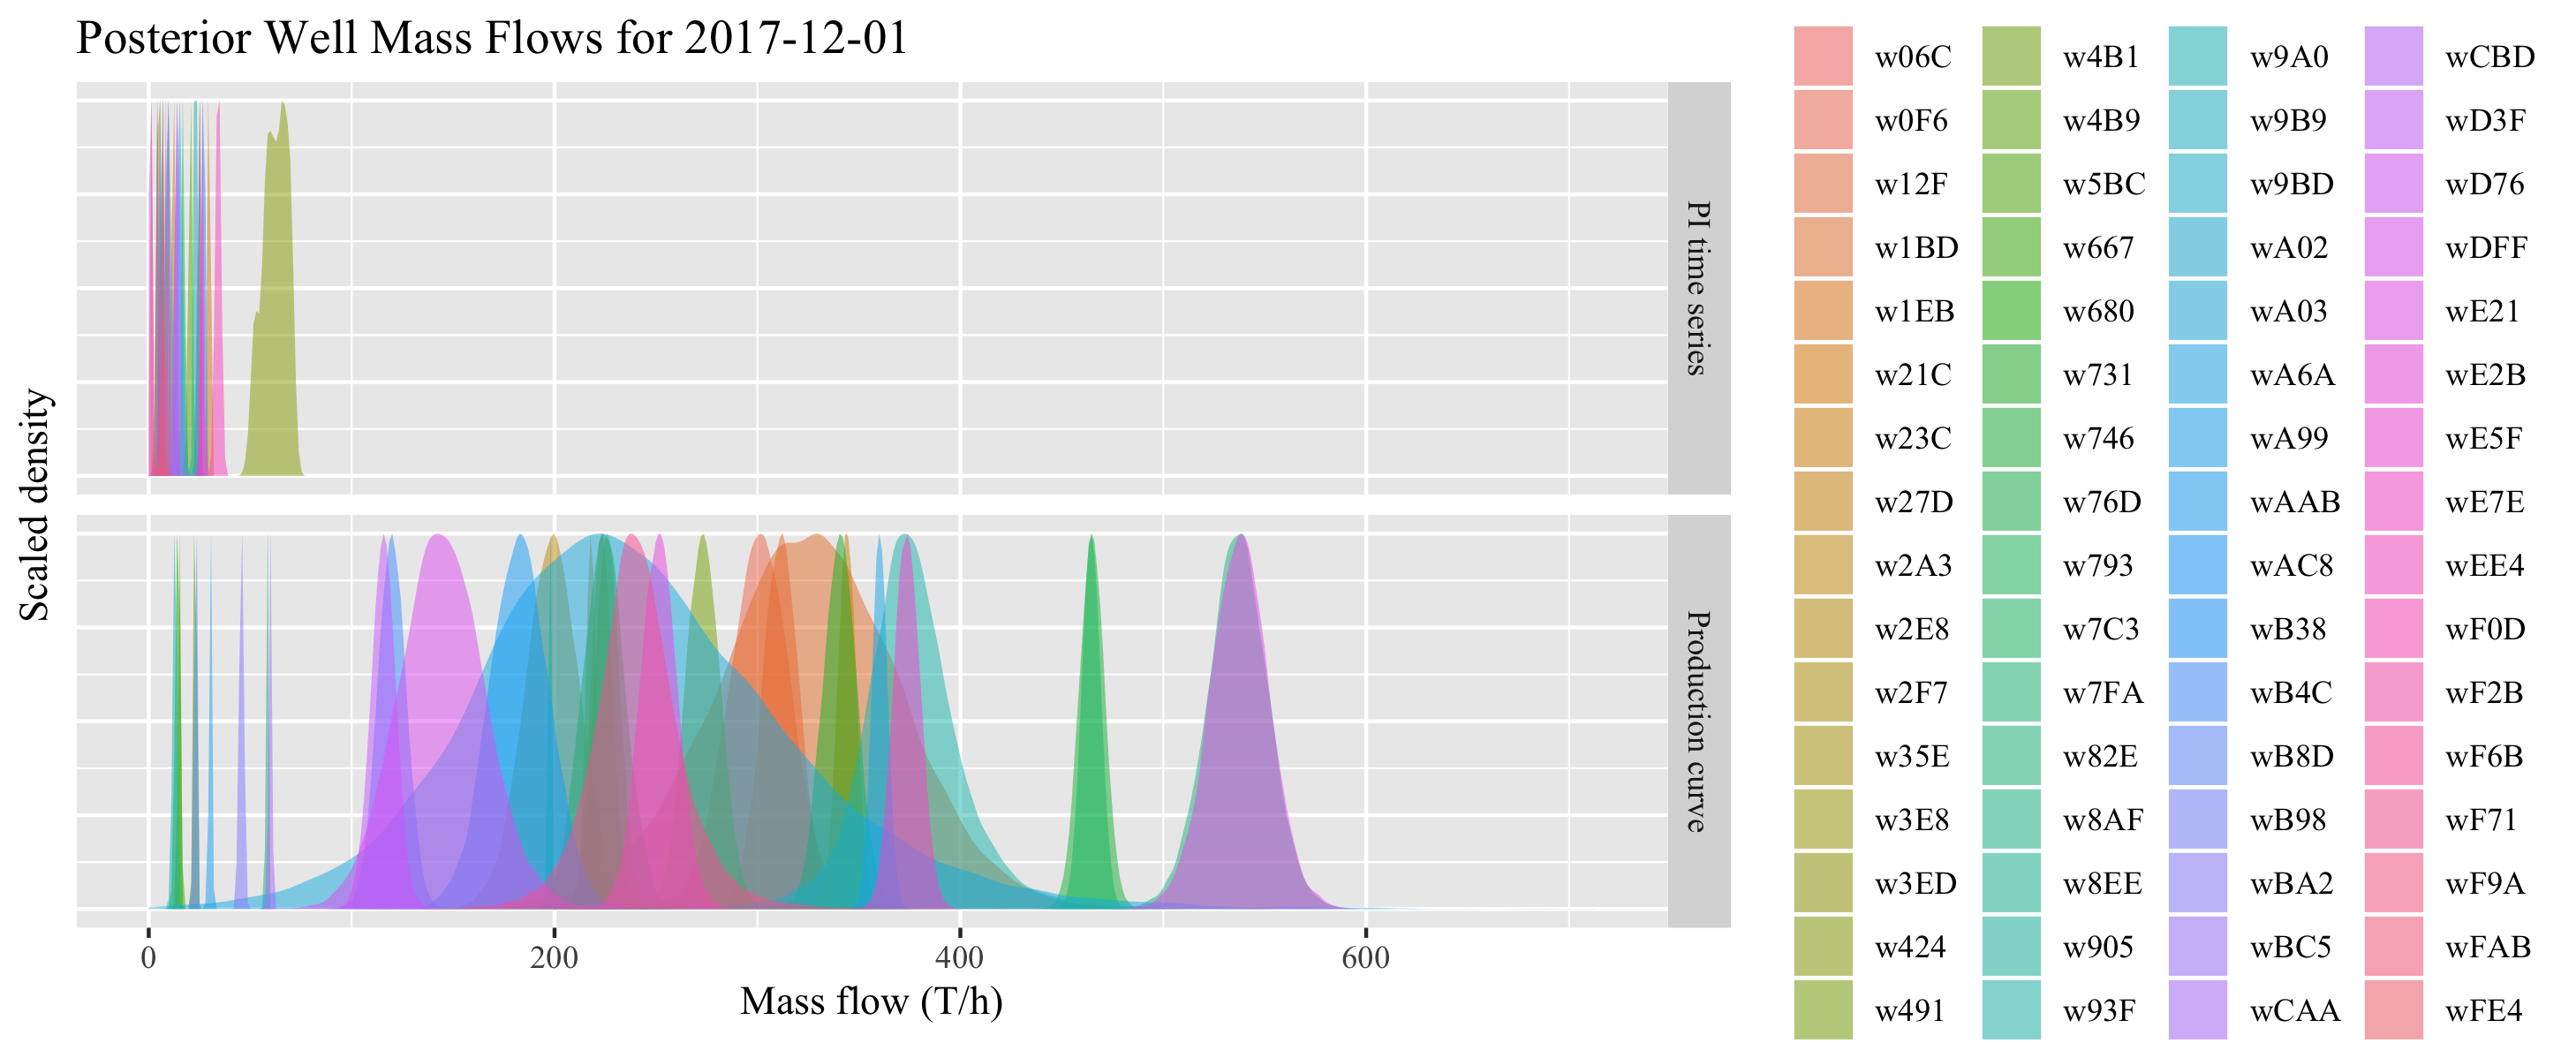
\includegraphics[width=\linewidth]{media/mf_wells}
  \captionof{figure}{Posterior mass flows, divided into wells with production curves and wells with a simple time-series (see Figure \ref{fig:ts_experiment} for time-series examples)}
  \label{fig:mf_wells}
\end{figure}

Figure \ref{fig:mf_wells} presents the posterior densities for mass flow at selected wells. We can see that some wells have more variation than others. The wells with low variance tend to be wells supported with PI data, either because they are dry wells, or they are liquid wells with mass flow meters. This is as expected because we have more information on their production characteristics and the information we have is also very close to our prediction date. The wells displaying large spread have some or all of the following issues:

\begin{enumerate}
\item Lack of data to fit the regression.
\item Data is for pressures and times far away from the values used for prediction; e.g. very old data that is no longer relevant.
\item Highly variable mass flow in some wells.
\item Mass flow is non-linear with pressure and time (i.e. bad fit).

\end{enumerate}

\subsection{Individual Well Declines}

\begin{figure}
  \centering
  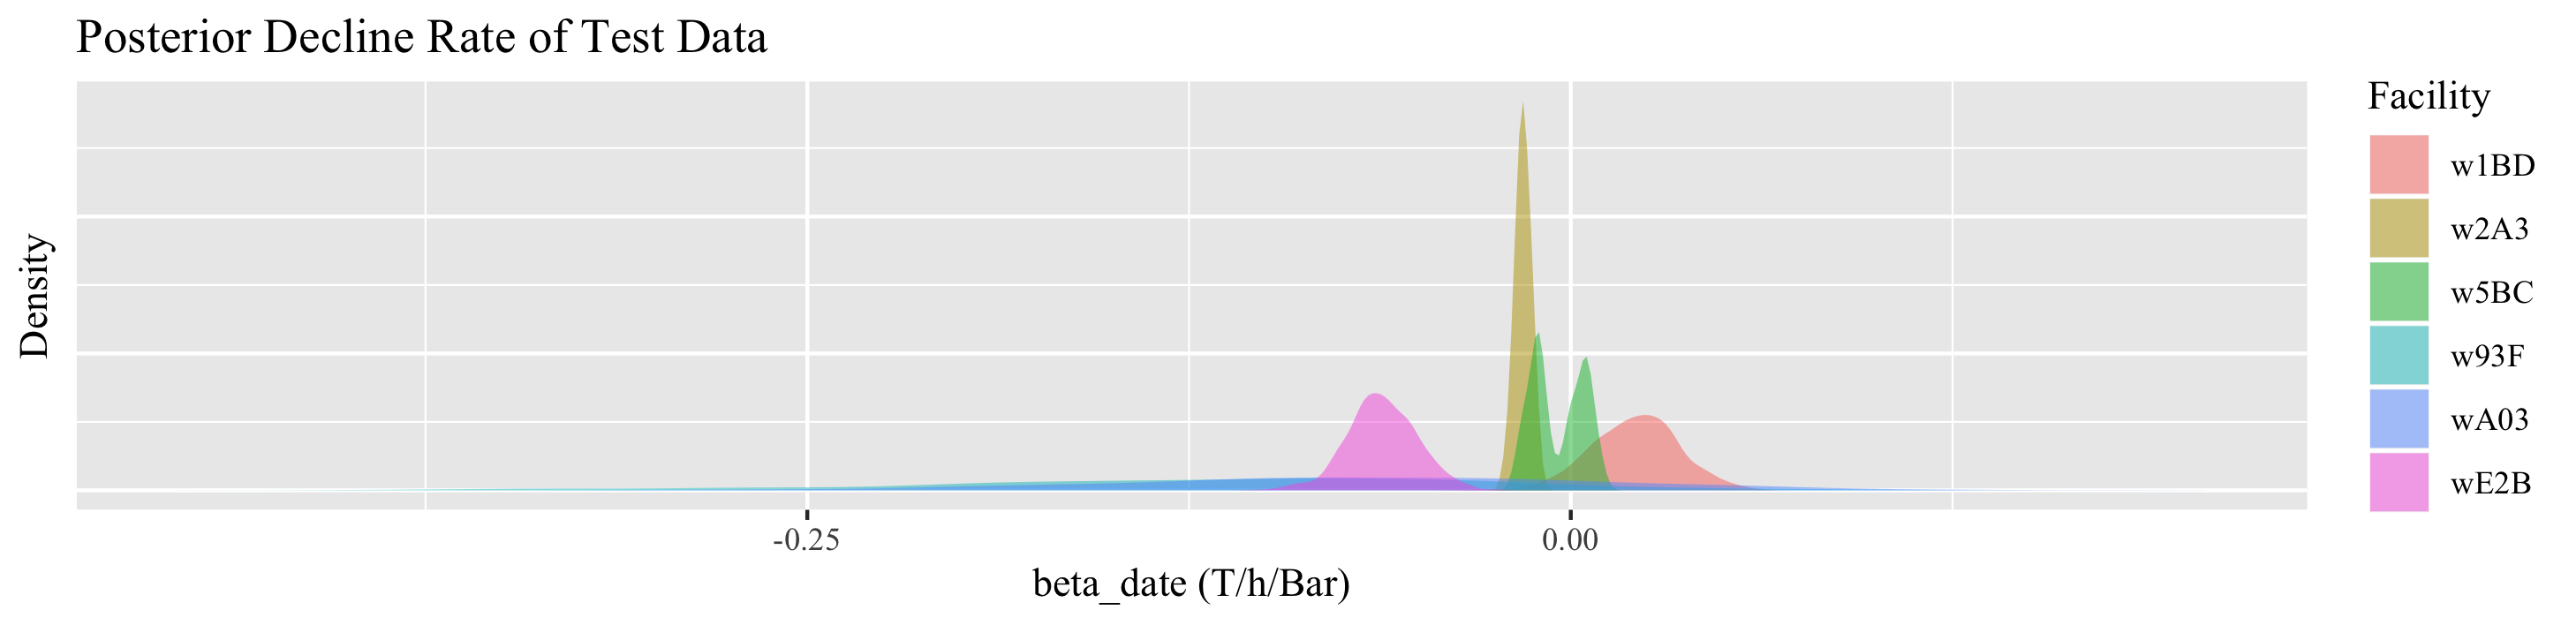
\includegraphics[width=\linewidth]{media/beta_date}
  \captionof{figure}{Posterior decline rate of selected liquid wells.}
  \label{fig:beta_date}
\end{figure}

% latex table generated in R 3.4.2 by xtable 1.8-2 package
% Thu Sep 20 12:22:42 2018
\begin{table}[h]
\centering
\begin{tabular}{lrrrr}
  \hline
well & Mean & Lower 2.5\% & Upper 97.5\% & n \\ 
  \hline
w06A & -0.021 & -0.039 & -0.000 &   10 \\ 
  wA2E & -0.272 & -0.332 & -0.214 &   88 \\ 
  wF8E & 0.010 & -0.035 & 0.048 &    4 \\ 
   \hline
\end{tabular}
\caption{Credible intervals for $\beta_\text{date}$ in units T/h/d. $n$ is the number of test data points rather than the total including PI data, because PI data is from a single month and cannot estimate the $\beta_\text{date}$ parameter on its own. Full table in Table \ref{tab:beta_date_all}.} 
\label{tab:beta_date}
\end{table}


Table \ref{tab:beta_date} presents credible intervals for decline at selected wells. The liquid wells have declines between zero and -0.2 T/h/d for a fixed well-head pressure, but some declines are not statistically significant, such as WK242.

There is varying precision -- WK263 is an example of a well with good precision in the decline rate. This is because there have been 34 recorded values with a range of covariate values, giving the parameter estimates good support.

Inspection of wells with poor precision in the regression parameters show that there is insufficient well test data available. For instance, WK270 has five points; this is not enough to estimate variance with three parameters.

\subsection{Flow Variances}
We may be interested in the flow variance or standard deviation -- how much it fluctuates with estimated measurement error removed. What does this mean JAGS models parameterise precision, but standard deviation  is usually more interpretable.

Focusing on the wells with sufficient sample sizes, we find that standard deviation differs between wells. Our posterior belief shows that WK242 has significantly higher variation than WK263.

\subsection{Down-flow Results}
The results from the previous section propagate through the network to the flash plants and generators. We are most interested in the flash plants, where we have an example spreadsheet of flows for a particular day and constraints on steam flows .

\subsubsection{Flash Plant Flow Verification}

\subsubsection{Flash Plant Constraints}
Contact Energy defines constraints on the flows in the network. We can estimate the probabilities of each constraint being violated by the proportion of the trace exceeding the constraint value. However, a more nuanced comparison can be made by the user in a density plot with the constraint value added.

\begin{figure}
\centering
  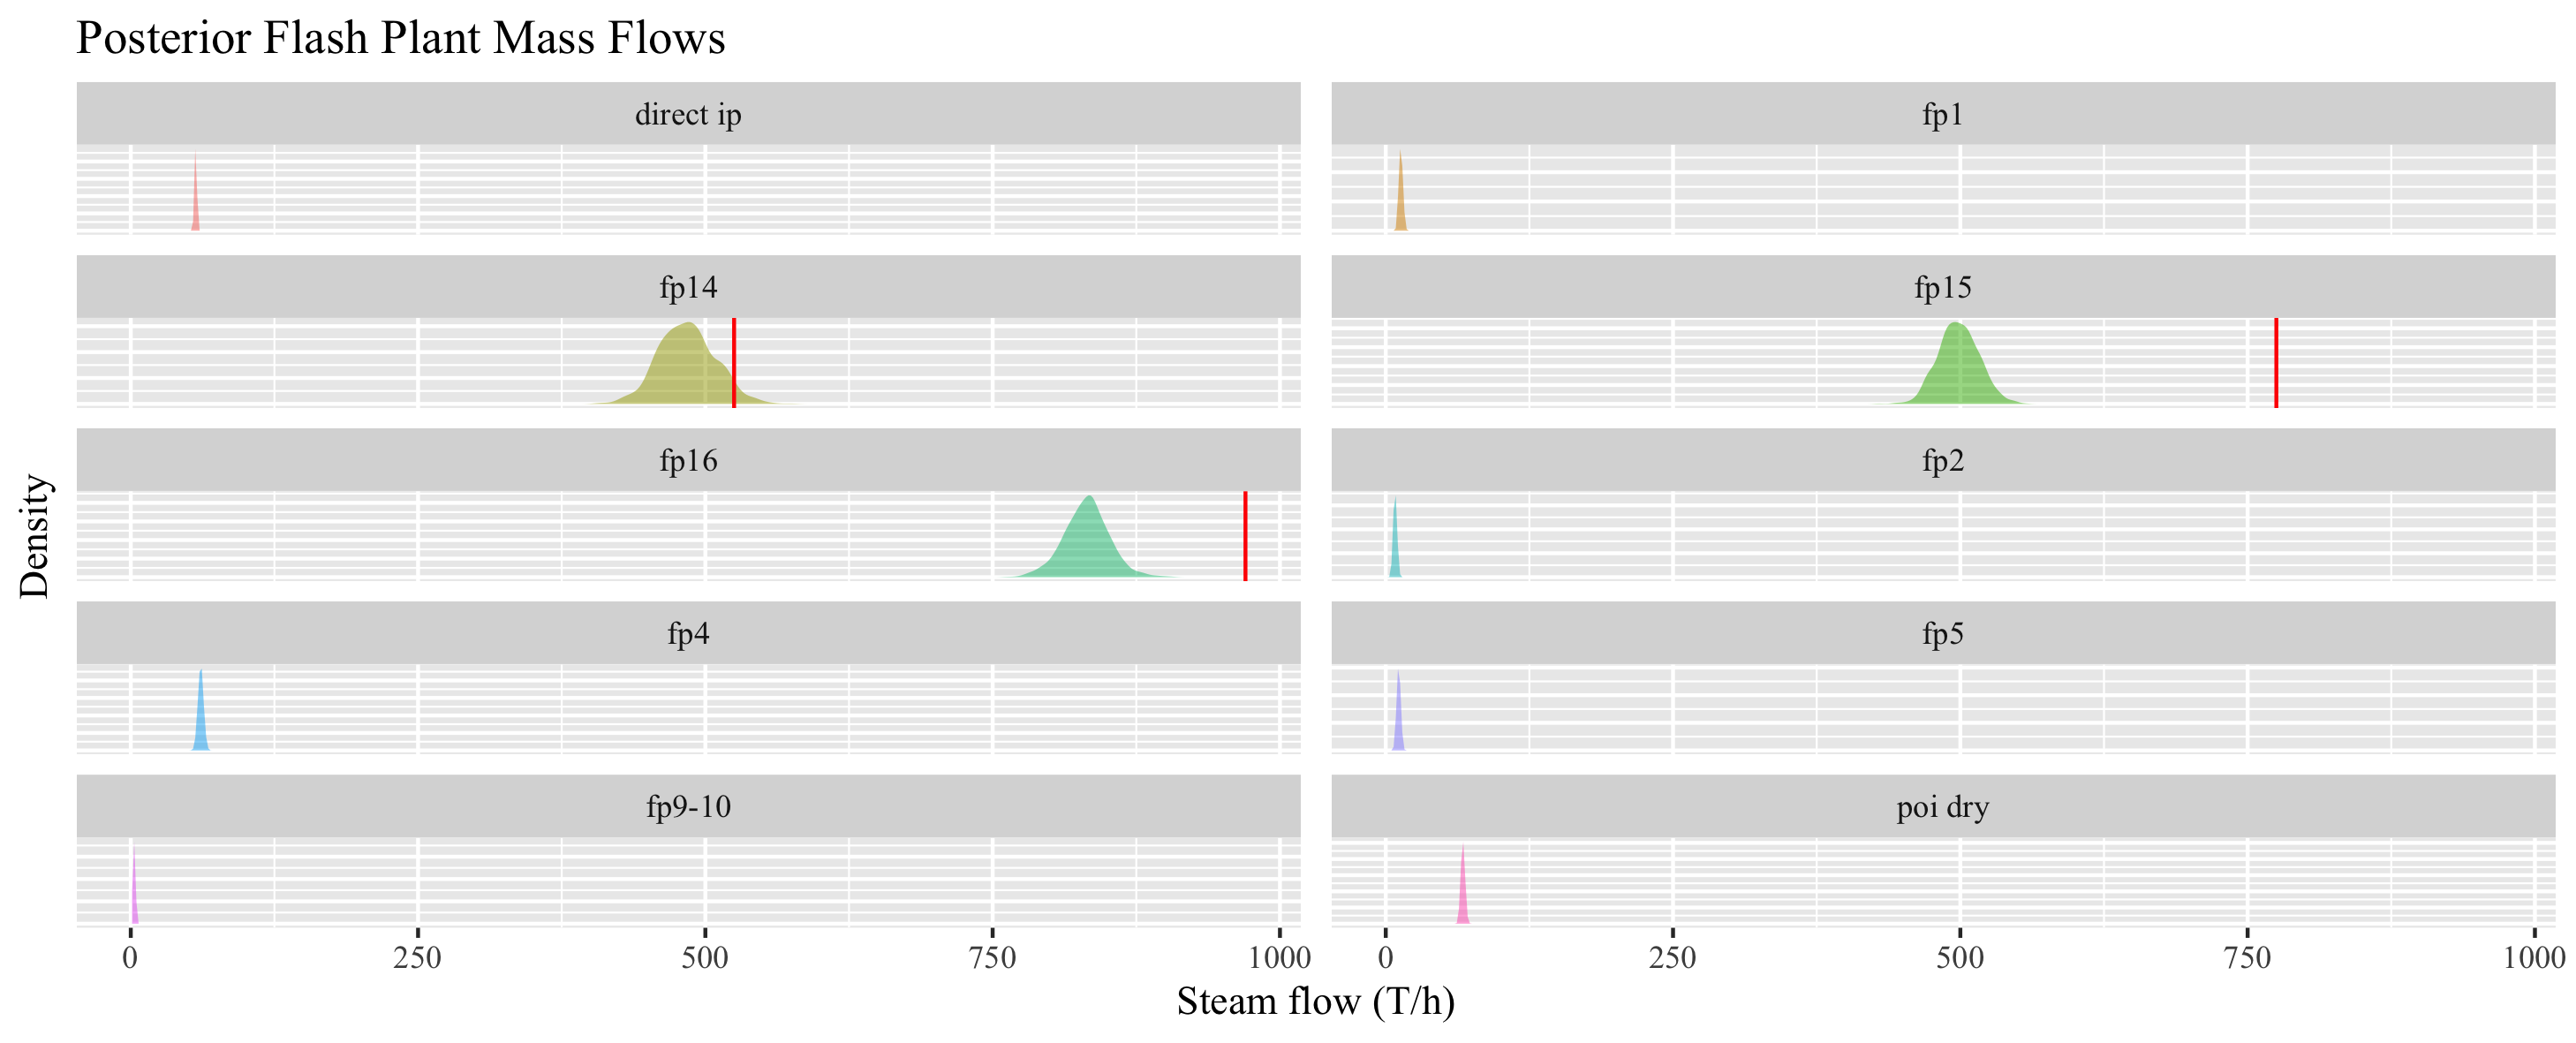
\includegraphics[width=\linewidth]{media/constraints}
  \captionof{figure}{Posterior density plot of the steam flows through the flash plants. Known steam limits are shown by a vertical red line.}
  \label{fig:constraints}
\end{figure}

Some of the flows are under-estimated because data is not available for all wells. However, in Figure \ref{fig:constraints} we can see that all of the flash plants are likely operating below their limits in the December 1st configuration. However, one flash plant is more likely to violate its constraints than the others, suggesting that one or more wells should be redirected to another flash plant.

We now reach the generators. Again, we only receive mass flows from wells we have data for, so the sums at the generators are incomplete.

\emph{(SEE APPENDIX. TODO Comparison shows that FPs feeding from liquid wells (with production curves) do not do very well. Therefore the production curves should not be used for day-to-day forecasting)}\todo{Comparison with PI data}

%%%%%%%%%%%%%%%%%%%%%%%%%%%%%%%%%
\section{Conclusions}
In this report, we show a hierarchical regression model and a directed network with uncertainty can be implemented in a single Bayesian model to estimate the true state of a geothermal surface network. Our model includes estimates of errors in both the steady-state properties of the network such as flows, and in the regression parameters such as production decline in the wells. Incorporating rates of decline allow us to make forecasts for dates beyond what the data covers. We have data until the end of 2017, so we make forecasts for 2018 (current date).

We also compare our posterior beliefs of the network against constraints set by the field's operators, and find that our simulation is able to probabilistically verify whether those constraints are violated in a given network configuration, as long as we have some data about the wells feeding a facility.

We find that almost all of the wells we analysed are in decline, and confirm that a regression model should fit separate parameters to each well because each well has a unique production curve and decline. Despite Contact Energy and Grant \& Bixley using an elliptic or otherwise curved model in their regression, we did not find significant evidence that the data would be better suited by a non-linear model.

To operate the model, we provide a configuration spreadsheet where the well/flash-plant and flash-plant/generator connectivity is specified, either as the output of an external third-party optimisation algorithm or as part of scenario analysis. This spreadsheet is also where constants such as enthalpy are specified.

In our parameter uncertainty analysis, we find that some regressions give us precise posteriors that contribute to good precision further down the network. In cases where there have been very few tests conducted for some wells, our estimates are less precise, and some of the liquid wells have no test data readily available. High variance in our estimates for well parameters gives an indication for which wells should be targeted by well testing to improve the accuracy of the model.

\todo{Note about performance and use cases -- should it be used}

%%%%%%%%%%%%%%%%%%%%%%%%%%%%%%%%%
\section{Further Development}
There are many opportunities to expand on the utility of this work.

\subsection{Direct Data Integration}
In this work, all data was obtained through Excel workbooks, even though some of it was originally stored in a PI system. Direct integration with the PI database would have benefits:

\begin{enumerate}
\item Automatic updates with daily data can track changes in trend as they happen within 24 hours.  We aimed to create a system that could deliver results within minutes instead of the considerable it takes to operate the Excel sheet, but this is only relevant if it is not delayed by the data source.
\item Data in the PI system is better structured because it is an automatic logger. We had to remove some data because of incompatibility with how it was stored, whereas a structured database would give us access to data points on more of the network facilities.
\end{enumerate}

\subsection{Time Series}
In our implementation of well declines, we treat measurements independently with respect to time. However, measurements are almost never truly independent and are often auto-correlated with previous measurements. Extra pre-processing to include auto-regression and differencing in the JAGS model is a common technique although it is difficult with irregularly spaced multivariate time series. Implementing non-independent time-series analysis will result in reduced standard errors.

\subsection{Prior Specification}
More prior specifications for parameters will add extra educated bias to our model, helping with variance reduction. Priors can be added to the hierarchical parameters on the regression coefficients, which are currently non-informative. For instance, if we knew an overall production decline rate and variance in decline across the field.

\subsection{Hierarchical Model Resolution}
Partitioning of components by manufacturer's specifications or age/generation will improve the hierarchical model. We currently treat all wells or flash plants as coming from the same family of facilities. However, we know the Wairakei geothermal field was built in a series of stages and that some facilities are more similar than others. Each family of facility should have its own hierarchical model, reducing variance in the hyper-parameters.

\newpage
\begin{appendices}
\section{Time Series}

\begin{figure}[h]
  \centering
  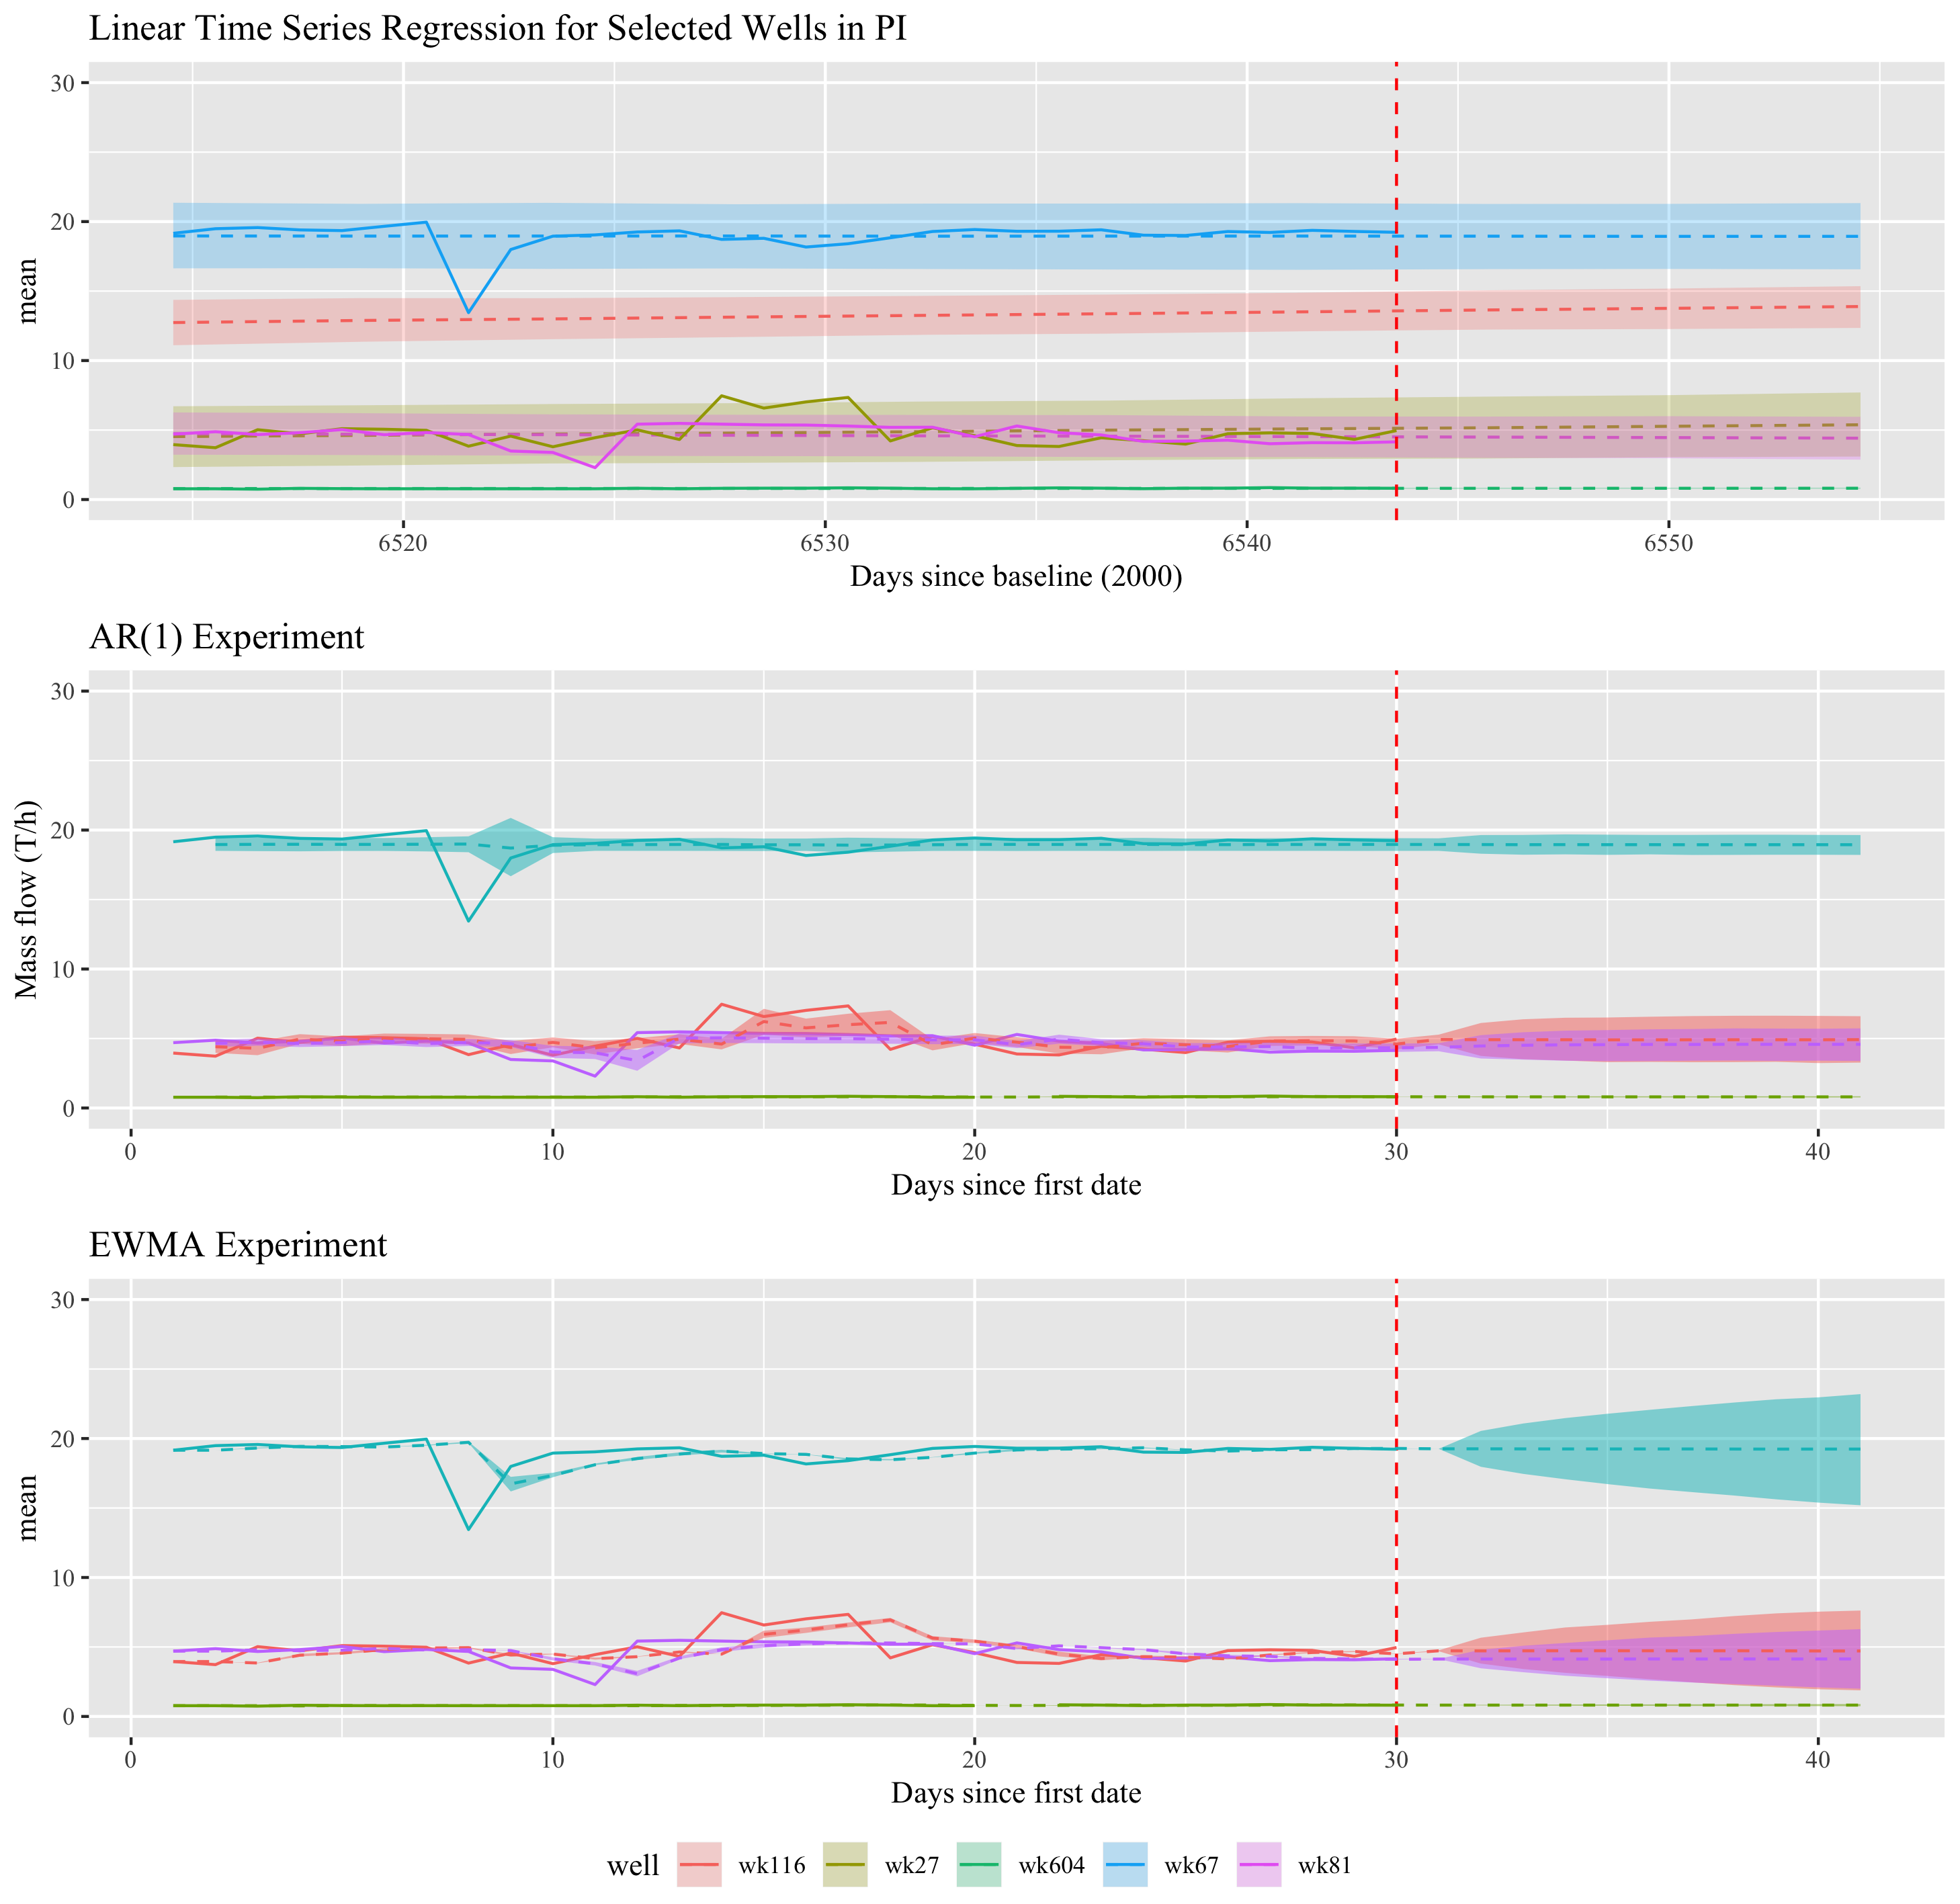
\includegraphics[width=\linewidth]{media/ts_experiment}
  \captionof{figure}{Time-series techniques on data from the PI database. We use the linear time series regression (top) for its robustness to systematic changes in operation, which cause the other regressions to become unstable.}
  \label{fig:ts_experiment}
\end{figure}

\newpage
\section{Verification}

\begin{figure}[h]
  \centering
  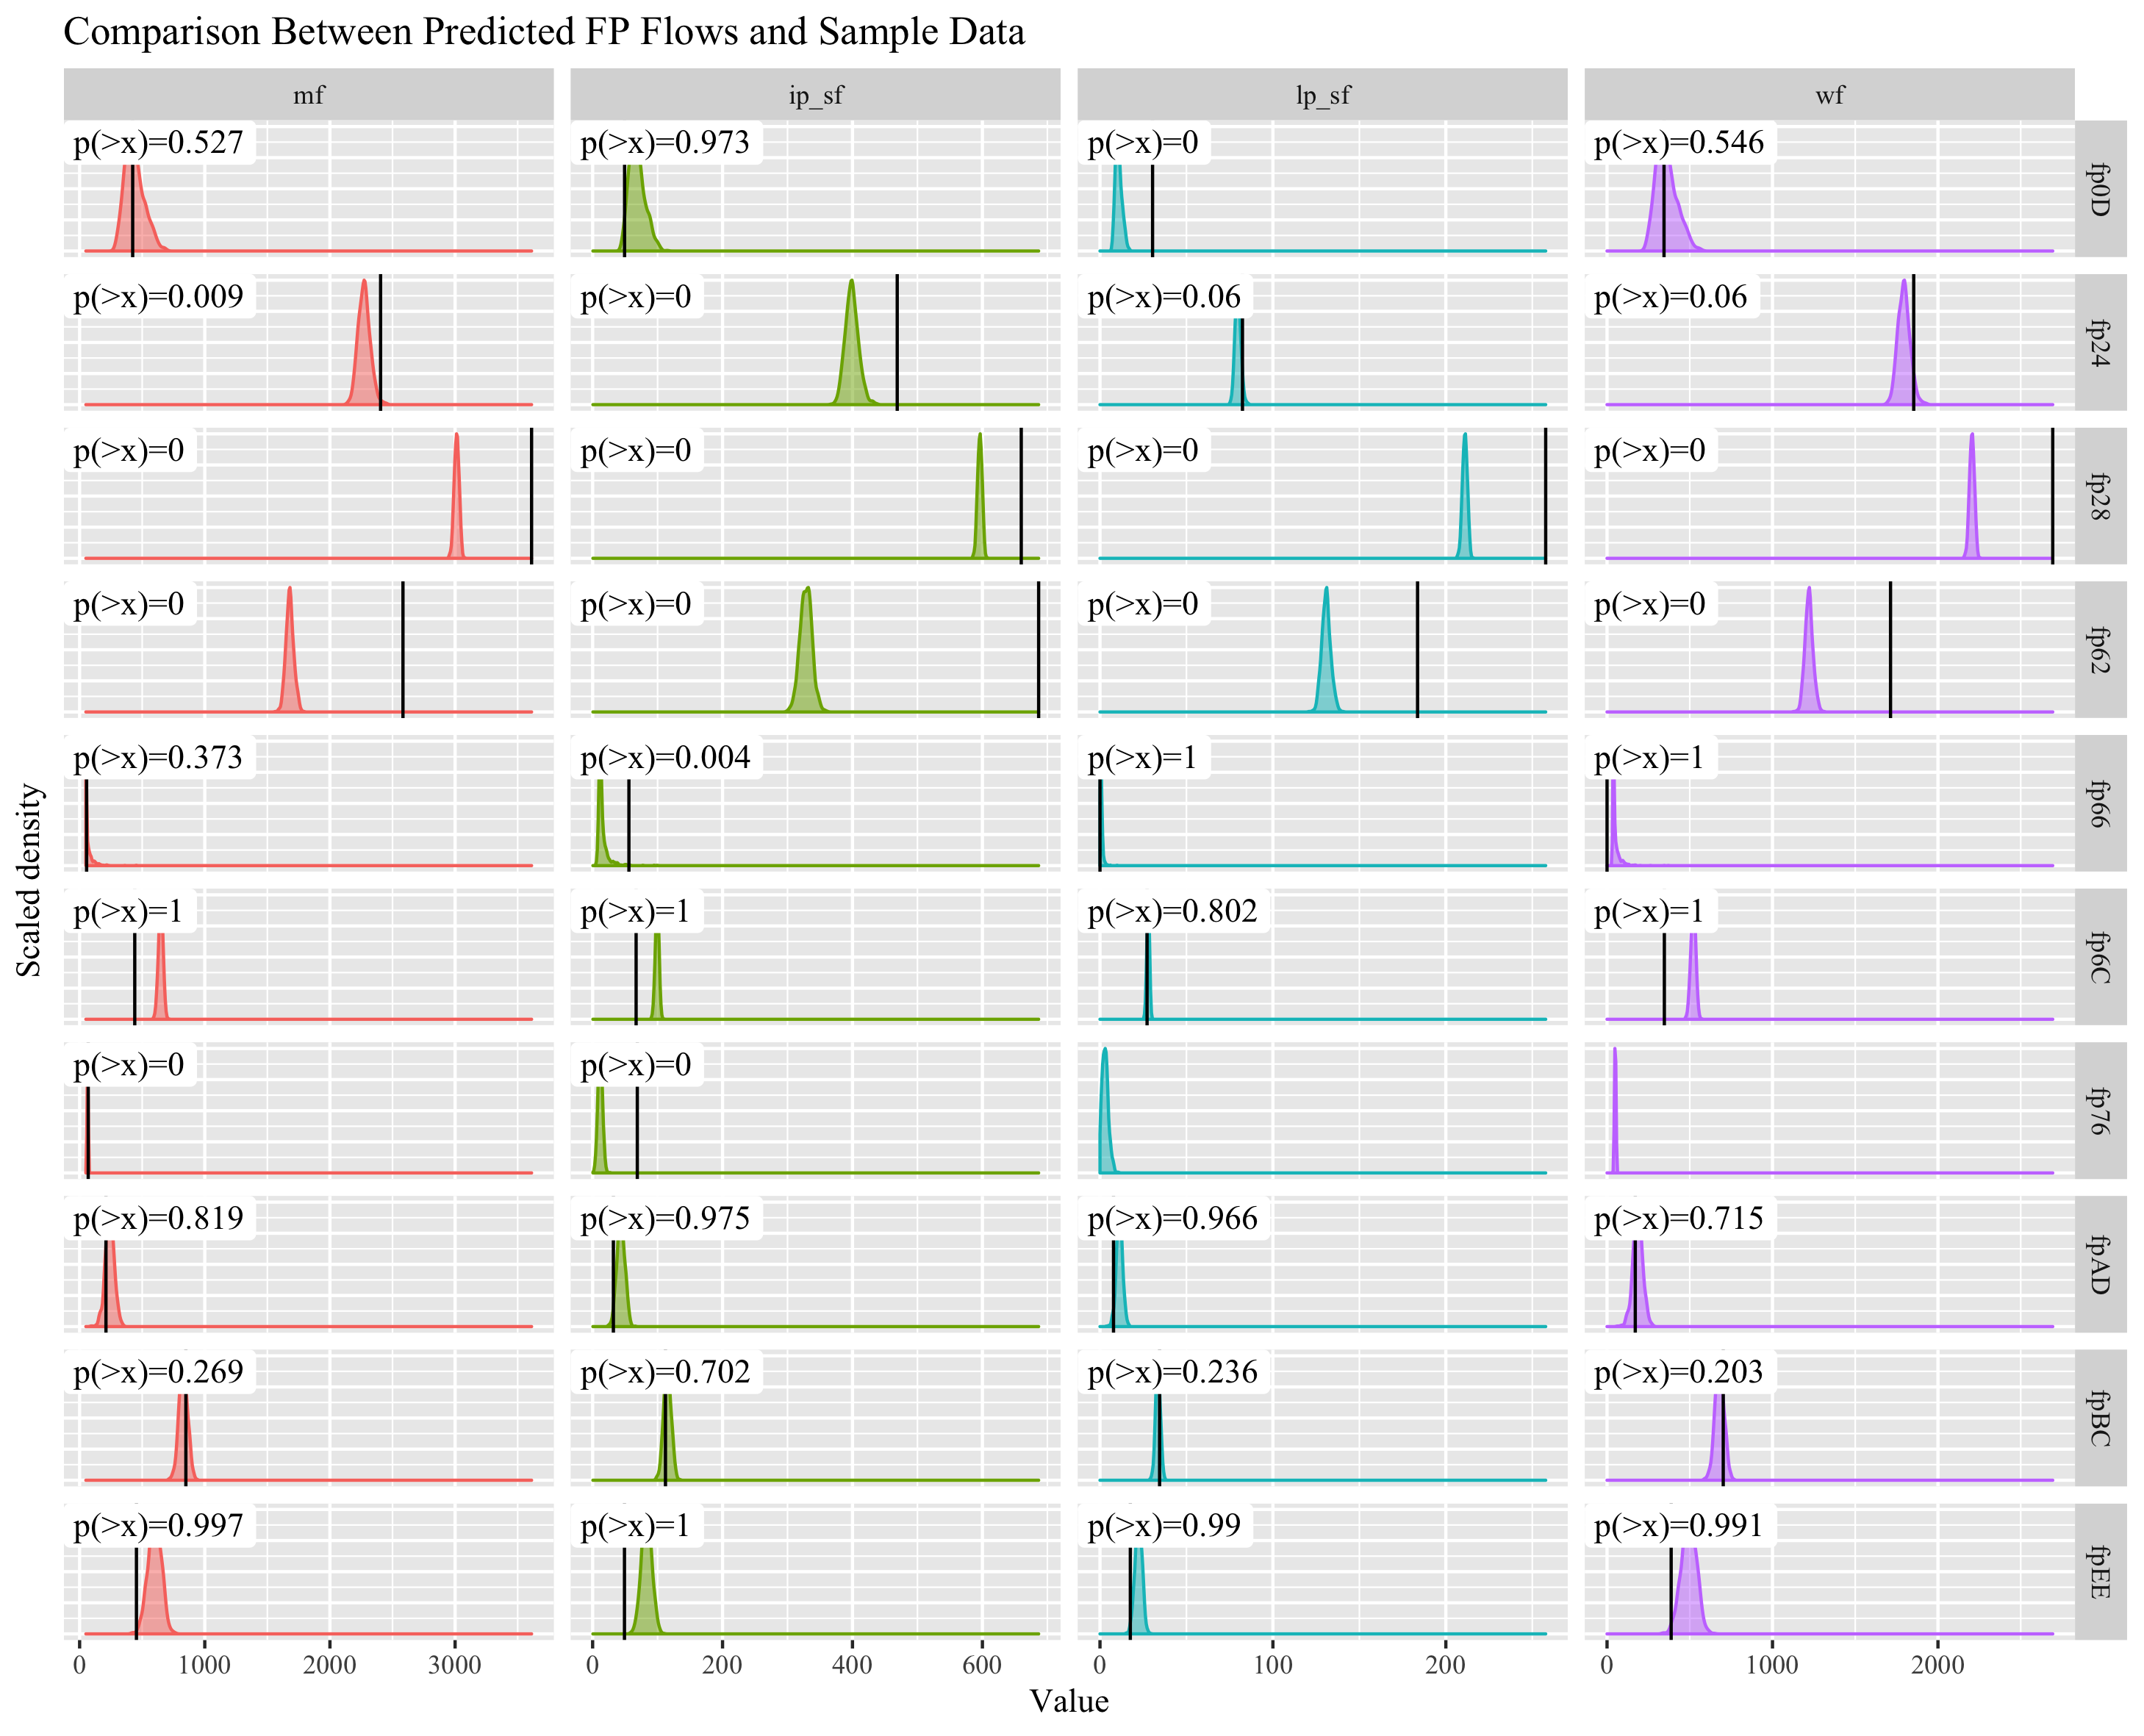
\includegraphics[width=\linewidth]{media/verification}
  \captionof{figure}{Verification of predicted flows with Excel shows a systematic deviation. Densities are the model predictions and black lines are the given figures from CEL (estimated by CEL, not direct from the PI loggers).}
  \label{fig:verification}
\end{figure}

\end{appendices}

\end{document}